\documentclass[twoside,11pt]{article}
\usepackage{graphicx}

%\usepackage[latin1]{inputenc}
\usepackage[utf8]{inputenc}
\usepackage[spanish]{babel}
\usepackage{amsmath, amsthm, amsfonts}
\usepackage{textcomp}
\usepackage[T1]{fontenc}
\usepackage{hyperref}
\usepackage{array}
\usepackage{MnSymbol}   % Para poder escribir el cuadrado negro

\usepackage{geometry}
    \geometry{a4paper,total={210mm,297mm},left=35mm,right=30mm,top=30mm,bottom=30mm,}

\usepackage{listings}
\lstset{
	% linewidth=15cm,
	% xrightmargin=1cm,
	breaklines=true,
	numbers=left,
	language=Matlab,
	frame=single}
\usepackage{color}
\usepackage{pgfplots}
\usepackage{pgfplotstable}
\usepackage{slashbox}
\usepackage{tikz}
\usetikzlibrary{arrows,shapes,trees}
\usepackage{multirow}

\usetikzlibrary{decorations.pathmorphing,patterns}

\renewcommand{\baselinestretch}{1.3}

\title{\begin{center} 

\includegraphics[scale=0.3]{images/upc.jpg} 
\end{center} 
\vspace{1cm} 
Proyecto Final de Carrera\\
INGENIERÍA INDUSTRIAL \\
\vspace{1.5cm} 
\Huge{Control de un Quadcopter} 
\vspace{0.5cm} \\ 
Memoria}
%\author{Gabriel de la Cal Mendoza}
\date{}

\usepackage{fancyhdr}		%% Para cabezera de página

\pagestyle{fancy}

% \lhead[x1]{x2}
% \chead[y1]{y2}
% \rhead[LE,RO]{z2}
% \renewcommand{\headrulewidth}{0.5pt}

% \lfoot[a1]{b2}
% \cfoot[c1]{d2}
% \rfoot[LE,RO]{
\includegraphics[scale=0.1]{etseib.jpg}}
% \renewcommand{\footrulewidth}{0.5pt}

\fancyhead[LO,RE]{Quadcopter Control}
\fancyhead[LE,RO]{\thepage}
\fancyfoot[LE,RO]{
\includegraphics[scale=0.2]{images/etseib.jpg}}
\fancyfoot[C]{}

\begin{document}
\maketitle
\begin{center}
\large{
$\begin{array}{ll}
\mbox{Autor:} & \mbox{Gabriel de la Cal Mendoza} \\
\mbox{Director:} & \mbox{Manel Velasco Garcia} \\
\mbox{Convocatoria:} & \mbox{Fecha a presentar}
\end{array}$}
\\ \vspace{2cm} \Large{Escola Tècnica Superior d'Enginyeria Industrial de Barcelona}\\ \vspace{1cm}

\includegraphics[scale=0.4]{images/etseib.jpg}
\end{center}

\thispagestyle{empty}
\newpage
\begin{center}

\end{center}
\thispagestyle{empty}
\newpage
\setcounter{page}{1}

\section*{Resumen}

En el presente proyecto se ha tenido como meta el control de un Quadcopter cuyas piezas se han adquirido por partes. Para tal propósito se ha linealizado  el modelo no lineal obtenido y controlado mediante un Regulador Lineal Cuadrático (LQR). El contenido de este trabajo está organizado en 8 secciones y 4 anexos.\\

En la sección \ref{prefacio} se presentan los motivos por el que la elección del tema de este PFC queda justificada. También se mencionan requerimientos previos que se han requerido para no tener insalvables dificultades. 

En la sección \ref{intro}, como Introducción, se hace un estudio del arte, con breves pinceladas del basto campo que hoy en día se encuentra sobre este tema. Además se describen los objetivos de este proyecto. Éstos no son más que el resolver todo problema que haya surgido durante esta aventura.

Se obtiene el modelo a partir de los parámetros característicos del sistema físico en la sección \ref{def}. En linealizar el sistema en el punto de equilibrio se llega a la conclusión de que las variables que lo forman se desacoplan y se comportan como un conjunto de dobles integradores. Ésto permite que la ley de control sea sencilla y justifica el que se hayan usado controladores basados PID tan asiduamente. También se presenta el modelo implementado en Simulink, con el que se probará el control obtenido posteriormente para verificar su eficiencia.

La sección anterior permite que en la \ref{control} se obtengan las acciones de control $u=-k \cdot X$ por medio de un LQR (Linear Quadratic Regulator). Se ataca al sistema con la ley obtenida juzgando los resultados.

En la sección \ref{implement} se explica cómo y qué se ha implementado respecto al control. Se comenta el código C que se está continuamente ejecutando.

En la sección \ref{construc} se describe tanto los componentes que se utilizan como el proceso de montaje paso a paso. Se justifica la elección de cada elemento tomando como criterio tanto las características de otros elementos como el dimensionado mismo del Quadcopter. 

En las secciones \ref{economics}, \ref{impacto} y \ref{conclusiones} se tiene un análisis económico, un estudio de impacto ambiental y las conclusiones respectivamente. En el primero se desglosan los costes materiales y se valoran las horas invertidas, considerando que el trabajo lo realiza un estudiante. En el estudio del impacto ambiental se describen los efectos en el medio ambiente de los componentes que se utilizan, tanto en la producción como en el reciclado. En la última sección se relata con qué se queda uno en limpio tras acabar esta empresa y cómo se espera continuar para futuros desarrollos.\\

En el Anexo 1 explica mediante código Matlab de dónde se ha extraído el vector de fuerzas del modelo. De esta manera se justifica la linealización en ser toda otra opción, en estas circunstancias, inviable.

En el Anexo 2 se detalla el proceso de grabado y posteriores modificaciones realizadas en el sistema operativo utilizado (Raspbian), para condicionar la Raspberry Pi tal y como se ha hecho para el Quadcopter.
 
En el Anexo 3 se describe qué es un filtro de Kalman, por qué es necesario y cómo se ha implementado. 

En el Anexo 4 se describe cómo se han caracterizado los motores y cómo se han obtenido sus curvas características de fuerza y consumo. 

\newpage
\begin{center}

\end{center}
\thispagestyle{empty}
\newpage

\setcounter{page}{1}
\tableofcontents
\addcontentsline{toc}{section}{Resum}
\fancyhead[LE,RO]{3}
\fancyfoot[C]{}
\newpage
\fancyhead[LE,RO]{\thepage}
\setcounter{page}{4}
\listoffigures
\newpage

\section{Prefacio} \label{prefacio}
\subsection{Motivación}

La principal motivación de este proyecto es la de aplicar por uno mismo los conocimientos básicos adquiridos en la carrera, y más en particular en el área del control en haber cursado la intensificación de automática.\\

En plantear un tema para el proyecto rápidamente surgió la idea de realizarlo sobre el control de un sistema mecánico, y más en particular sobre uno que estuviera actualmente emergiendo tanto en mercados como en el campo de la investigación.\\ 

De entre las diferentes alternativas, un quadcopter es la más atractiva para el proyecto tanto por su simplicidad constructiva como por su no excesivo coste. Existen actualmente en el mercado infinidad de proveedores para los componentes necesarios para construir un quadcopter, con un gran abanico de opciones de entre las que escoger cada elemento como motores, baterías, electrónica, etc.\\

Las posibles aplicaciones son numerosas, tanto que aún no se han ni tan solo explotado todas las posibles. Como ejemplo: vigilancia de superficies abiertas, transporte de pequeños paquetes, herramienta de ocio, entre otras.\\

Entender el funcionamiento y familiarizarse con el mecanismo es una inquietud que se ha mantenido insatisfecha durante largo tiempo. Con este pretexto se pretende acabar de justificar la elección del tema de ésta pequeña gran empresa.

\subsection{Requerimientos previos}

Es necesario tener ciertos conocimientos mínimos en automática para poder controlar el quadcopter, así como la inquietud de aprender lo que sea necesario para cumplir, en la medida de lo posible, los objetivos iniciales del presente proyecto. \\

Nociones de mecánica son necesarias para elaborar e interpretar el sistema sobre el que se trabaje, así como sus resultados. Conocimientos del lenguaje $C$ son imprescindibles ya que el código del programa que realiza los cálculos está escrito en este mismo lenguaje. 

Para adaptar los elementos que componen el aparato y afianzarlos a la estructura (Frame)  del Quadcopter ha sido de gran ayuda contar con el servicio de una impresora 3D, creada por uno mismo. Finalmente, estar familiarizado con el argot y elementos de un Quadcopter, así como motores, emisoras de radio, entre otros es de ayuda. \\

Superar las dificultades que han surgido, teniendo en cuenta que el fin no justifica los medios, es la praxis que se ha aplicado a la hora de realizar éste trabajo. Finalmente, recordar reminiscencias de la carrera es siempre útil e interesante, así que conceptos adquiridos pero no utilizados se esperan aplicar.
 
\newpage
\section{Introducción} \label{intro}

Un Quadcopter es un vehículo volador no tripulado ($Unmanned \>Aerial\>Vehicle$ o $UAV$) que se caracteriza por tener quatro rotores a modo de actuadores en vez de dos como en el caso de los helicópteros. Este tipo de autogiro intenta obtener una flotabilidad estable y vuelo preciso balanceando las fuerzas producidas por los cuatro motores y surge de la necesidad de tener un aparato de vuelo de dimensiones reducidas y gran estabilidad, con prestaciones superiores a las de un helicóptero convencional. \\

\begin{figure}[h!]
\begin{center}
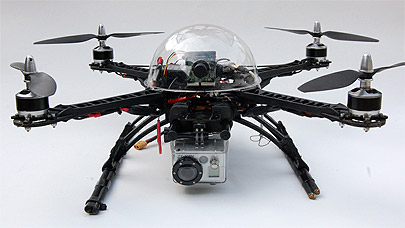
\includegraphics[scale=0.4]{images/quadcopter_example.jpg}
\caption{Quadcopter de ejemplo con cámara}
\end{center}
\end{figure}


Una de las ventajas que se obtiene con este cambio es la mayor capacidad de carga ya que es tienen 4 motores  para soportar el peso. La estabilidad del vehículo mejora en permitir aterrizajes y despegues verticales con una mayor maniobrabilidad. También puede trabajar en áreas de difícil acceso o más agresivas, como con lluvia y viento. \\

Esquemáticamente se puede representar como una estructura en $X$ con su centroide coincidiendo con el centro de masas i cuatro actuadores a las puntas de cada brazo, todos ellos apuntando en la misma dirección y sentido, pero con giros de aspa en sentido contrario, pero igual en lados opuestos.


\subsection{Estudio del arte}

En la actualidad el campo referente a estos aparatos se ha diversificado tanto que se pueden encontrar muchas variedades y tipos de Quadcopters. Se ha hecho mención del modelo de cuatro motores, pero bien pueden encontrarse de tres hasta 8 motores, sino más en casos más concretos. \\

\begin{figure}[h!]
\begin{center}
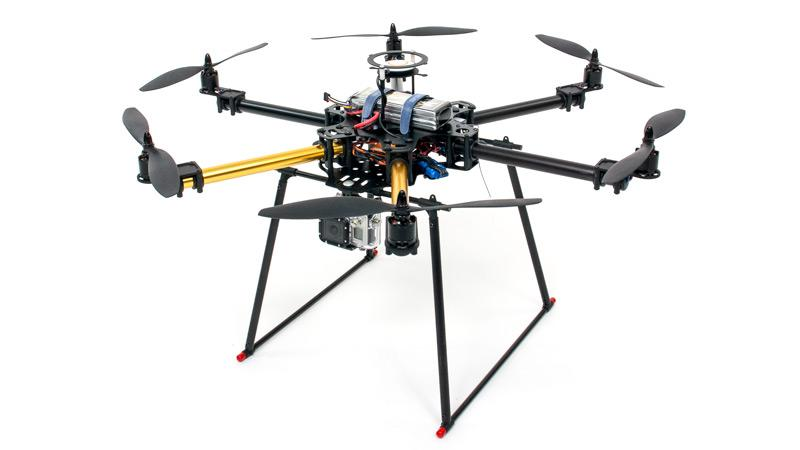
\includegraphics[scale=0.3]{images/6_armed_quadcopter.jpg}
\caption{Ejemplo de Quadcopter con 6 motores}
\end{center}
\end{figure}

Con el objetivo de desarrollar un $UAV$ que realice tareas de forma totalmente autónoma, se han diseñado sensores para estimar los estados del vehículo de manera más rápida y eficiente, así como diferentes estrategias para controlar la estabilidad y orientación del mismo. Se ha utilizado visión  por computador para realizar aterrizajes, detección de objetivos y navegación autónoma. También pueden combinarse diferentes técnicas con el uso del GPS para asegurar una buena orientación del aparato. \\

Para controlar esta clase de aparatos se utilizan diferentes leyes de control, así como PID, LQR, Redes Neuronales, Machine Learning, entre otros. La más utilizada es sin duda un PID por su fácil implantación y poca carga computacional.

\subsection{Objetivos del proyecto}

La meta que se persigue es la de hacer planear un Quadcopter en direcciones horizontales. A la vez, éste es un excelente subterfugio para cumplir con otros objetivos relacionados con este fin como el control de motores, el inteligente uso de la electrónica y correcto diseño mecánico del aparato. Además, se espera haber ampliado la visión que uno tiene en cada campo. \\

De entre todas las disciplinas involucradas, se espera acabar familiarizado con las facetas relacionadas con la presente empresa para clarificar la relación entre los elementos que componen un Quadcopter.  A saber, se espera poder acabar entendiendo la electrónica, mecánica y conocimientos de control que reinan en el sistema. \\

En el caso de la electrónica se espera entender y poder implementar sencillos protocolos de comunicación, en este caso $I2C$ entre los sensores y la Raspberry Pi. Ésta misma es el centro neurálgico del Quadcopter, así que es esencial saber utilizarla como se requiere para que pueda recibir consignas, estados y enviar la correspondiente acción de control a los motores para que se llegue al estado final deseado. \\

Por parte de la mecánica, es primordial tener conocimientos sólidos de conceptos como el Teorema de la Cantidad de Movimiento y el de la conservación del Momento de Inercia, así como poder calcular el Lagrangiano ($\mathcal{L}$) para generar un modelo verosímil y que represente fidedignamente la realidad para que se desarrolle de manera efectiva el control. \\

Finalmente, y como más serio objetivo de toda esta aventura, es el de haber afianzado lo que se creía entendido en relación al control. Asimilar otros métodos de control aplicables a sistemas multilineales no contemplados en la carrera es un excitante reto que se espera haber superado con éxito. \\

Entonces, se entiende este trabajo como la causa de la motivación a cumplir con un objetivo multidisciplinar como puede serlo cualquiera en el campo de la robótica, en el que se debe tener constancia de muchos aspectos relevantes, como el de la economía. Poder tener idea de lo que cuesta un robot es de gran importancia si uno se embarca en un proyecto de envergadura, ya que se quiere que los pronósticos sobre el presupuesto cuadren con la futura realidad. 

\newpage
\section{Definición del modelo} \label{def}
\subsection{Definición de les variables}
Para caracterizar la planta con la que es trabajará, es necesario obtener un modelo del Quadcopter. Las constantes propias del modelo se dejaran en forma de parámetros a calibrar una vez se tenga el objeto físico. De esta manera el modelo será general para todo quadcopter que comparta la misma familia de parámetros.
Es necesario considerar dos marcos de referencia: el inercial formado por los ejes $x,y,z$ y el del cuerpo (Body) formado por los ejes $x_B,y_B,z_B$. El primero tiene la perspectiva de el observador en tierra, estático, mientras que el segundo es solidario a la estructura. Según la orientación de los ejes del cos con esta referencia se pueden dar los siguientes dos casos:
\begin{itemize}
\item \textbf{Cross type}: Los ejes de coordenadas coinciden con los brazos de la estructura ya que se tienen los actuadores a las puntas de cada brazo.
\item \textbf{X-type}: Los ejes y la estructura forman $45º$. Se tienen entonces dos motores en la parte delantera y dos en la trasera.
\end{itemize} 
Por ser más usual la primera opción, se decide utilizar la configuración $Cross type$ tal y como se tiene en la figura \ref{RefQuad}.
\begin{figure}[h!]
\centering
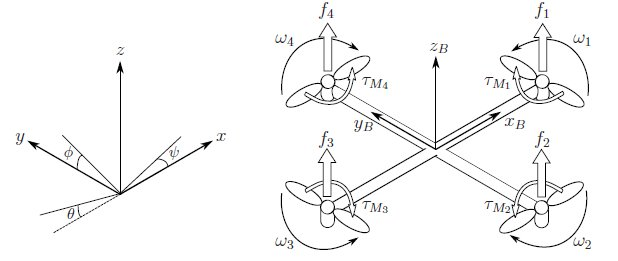
\includegraphics[scale=0.5]{images/quad.jpg}
\caption{Marcos de referencia en el quadcopter}
\label{RefQuad}
\end{figure}\\
Se supone que el objeto es un rotor esférico, y por tanto su tensor de inercia es diagonal:
\begin{equation}\textbf{I}=\left[ \begin{array}{ccc}
I_{xx} & 0 & 0 \\
0 & I_{yy} & 0 \\
0 & 0 & I_{zz} 
\end{array} \right] \end{equation}
Se define la posición lineal absoluta con las coordenadas $x,y,z$ con vector $\pmb{\xi}$ e igualmente para la posición angular a partir de $\pmb{\eta}$ según:
\begin{equation} 
\pmb{\xi}=\left[ \begin{array}{ccc}
x\\
y\\
z \end{array} \right] ,\quad \pmb{\eta}=\left[ \begin{array}{ccc}
\phi\\
\theta\\
\psi \end{array} \right] , \quad \pmb{q}=\left[\begin{array}{c}
\pmb{\xi}\\
\pmb{\eta} \end{array} \right] 
\end{equation}

donde $\phi$ es el ángulo de cabeceo (Pitch), $\theta$ és el de balanceo (Roll) y $\psi$ el de guiñada (Yaw).\\
Para la orientación angular entre los dos marcos se tiene un sistema de referencia con ángulos Tait-Bryan, donde la matriz de transformación es:
\begin{equation}
\pmb{R}=\left[\begin{array}{ccc}
C_\psi C_\theta & C_\psi S_\theta S_\phi - S_\psi C_\phi & C_\psi S_\theta C_\phi + S_\psi S_\phi \\
S_\psi C_\theta & S_\psi S_\theta S_\phi + C_\psi C_\phi & S_\psi S_\theta C_\phi - C_\psi C_\phi \\
-S_\theta & C_\theta C_\phi & C_\theta C_\phi 
\end{array}\right]
\end{equation}
con $C_\phi=cos(\phi)$ i $S_\phi=sin(\phi)$. Las velocidades lineales en el marco de referencia del cuerpo (Body Frame) se representen con el vector $v_B$ y las velocidades angulares con $\gamma$ según:
\begin{equation}
\pmb{v_B}=\left[\begin{array}{c}
v_{x,b}\\
v_{y,b}\\
v_{z,b}\\
\end{array}\right] \hspace{1cm} \pmb{\gamma}=\left[\begin{array}{c}
p\\
n\\
r
\end{array} \right]
\end{equation}
En cambio, las velocidades en el marco de referencia inercial (Inertial Frame)  se representan por $\dot{\eta}$ para las velocidades lineales y con $\dot{\xi}$ para las angulares: 
\begin{equation}
\pmb{\dot{\xi}}=\left[\begin{array}{c}
\dot{x} \\
\dot{y} \\
\dot{z}
\end{array} \right] \hspace{1cm} \pmb{\dot{\eta}}=\left[\begin{array}{c}
\dot{\psi} \\
\dot{\theta} \\
\dot{\psi}
\end{array} \right] 
\end{equation}
Ya que la derivada de los ángulos $\phi$, $\theta$ y $\psi$ no es el vector de velocidades angulares es necesario tener un cambio de base para relacionar el marco de referencia inercial con el del cuerpo con la matriz $W_\eta$:
\begin{equation}
\pmb{W_\eta}=\left[\begin{array}{ccc}
1 & 0 & -S_\theta \\
0 & C_\phi & C_\theta S_\phi \\
0 & -S_\phi & C_\theta C_\phi 
\end{array} \right] \hspace{0.5cm} amb \hspace{0.5cm} 
\pmb{\gamma}=\left[ \pmb{W_\eta} \right] \pmb{\dot{\eta}} 
\end{equation}
Las fuerzas de sustentación y velocidades angulares de los cuatro actuadores son $f_1,f_2,f_3,f_4$ i $w_1,w_2,w_3,w_4$ respectivamente. Siguiendo la orientación de la figura \ref{RefQuad}, con el objetivo de poder anular los momentos producidos en el eje $z_B$ (en el marco del cuerpo $B$) el sentido de giro de los actuadores  $4$ y $2$ son en el de las agujas del reloj (clockwise) y el de los $1$ y $3$ en sentido contrario (counterclockwise). \\

Interesa conocer qué fuerza y momento aportará cada motor dada una velocidad angular conocida. Se supone poder controlar la fuerza y momento ejercida por cada motor y cómo aproximación inicial se considera que están relacionados con la velocidad angular de la forma:
\begin{equation}
\begin{array}{l}
f_i=kw^2_i \\ 
\tau_{M_i}=bw^2_i
\end{array}
\end{equation}
Por tanto el empuje total $\pmb{T_B}$ proporcionado en la dirección $z_B$ y los momentos generados $\pmb{\tau_B}$ por los motores son:
\begin{equation}
\pmb{T_B}=k\left(\sum_{i=1}^{4}w^2_i \right)e_{z_B}=\left[ \begin{array}{c}
0 \\
0 \\
\displaystyle\sum_{i=1}^{4}f_i
\end{array} \right] 
\hspace{1cm} \pmb{\tau_B}=\left[ \begin{array}{c}
\tau_\phi \\
\tau_\theta \\
\tau_\psi
\end{array} \right] = \left[ \begin{array}{c}
l(f_4 - f_2) \\
l(f_3 - f_1) \\
\displaystyle\sum_{i=1}^{4}\tau_{M_i}
\end{array} \right]
\end{equation}

\subsection{Obtención del modelo}
Las ecuaciones que gobiernan el sistema se obtienen con el método de Euler-Lagrange, por lo que se empieza obteniendo el Lagrangiano del sistema:
\begin{equation}
\mathcal{L}=E_{cinetica} - E_{potencial} = (E_{translacion}+E_{rotacion})-E_{potencial}
\end{equation}

Substituyendo cada componente por su expresión:
\begin{equation}
\mathcal{L}(\pmb{q},\pmb{\dot{q}})=\frac{m}{2} \pmb{\dot{\xi}}^T \pmb{\dot{\xi}} + \frac{1}{2}\pmb{\gamma}^{T}\pmb{I}\pmb{\gamma} - mgz
\end{equation}
Es encuentra el vector de fuerzas y  momentos:
\begin{equation}
\pmb{F}=\left[ \begin{array}{c}
\pmb{f} \\
\pmb{\tau_B}
\end{array} \right] = \frac{d}{dt}\left(\frac{\partial \mathcal{L}}{\partial \pmb{\dot{q}}}\right)-\frac{\partial\mathcal{L}}{\partial \pmb{q}}
\end{equation}

amb $ \hspace{0.5cm} \pmb{q}=[\begin{array}{cccccc}
x & y & z & \phi & \theta & \psi
\end{array} ]^{T} \hspace{0.5cm}$ i $ \hspace{0.5cm} \pmb{\dot{q}}=[\begin{array}{cccccc}
\dot{x} & \dot{y} & \dot{z} & \dot{\phi} & \dot{\theta} & \dot{\psi}
\end{array} ]^{T}$.\\

En calcular $F$ es necesario hacer el cambio de variables de $\gamma$ a $\dot{\eta}$ con el cambio de base $\dot{\eta}=\left[ W_\eta \right]^{-1} \gamma$ para poder derivar el Lagrangiano respecto $\dot{q}$, que son las variables propias del marco de referencia inercial:

\begin{equation}
\frac{1}{2}\pmb{\gamma}^{T}\pmb{I}\pmb{\gamma} = \frac{1}{2}(\pmb{W_\eta} \pmb{\dot{\eta}})^{T}\pmb{I}(\pmb{W_\eta} \pmb{\dot{\eta}}) = \frac{1}{2}\pmb{\dot{\eta}}^{T}(\pmb{W_\eta} ^{T}\pmb{I}\pmb{W_\eta})\pmb{\dot{\eta}} = \frac{1}{2}\pmb{\dot{\eta}}^{T}\pmb{J}\pmb{\dot{\eta}}
\end{equation}

donde la matriz $J$ queda como
\begin{equation}
\pmb{J}=\pmb{W_\eta} ^{T}\pmb{I}\pmb{W_\eta} = \left[ \begin{array}{ccc}
I_{xx} & 0 & -I_{xx} S_\theta \\
0 & I_{yy} C^2_\phi + I_{zz} S^2_\phi & (I_{yy}-I_{zz}) C_{\phi} S_\phi C_\theta \\
-I_{xx} S_\theta & (I_{yy}-I_{zz}) C_{\phi} S_\phi C_\theta & I_{xx} S^2_{\theta}+I_{yy} S^2_{\phi} C^2_\theta +I_{zz}C^2_{\phi} C^2_{\theta}
\end{array} \right]
\end{equation} 

y por tanto el Lagrangiano queda:

\begin{equation}
\mathcal{L}(\pmb{q},\pmb{\dot{q}})=\frac{m}{2} \pmb{\dot{\xi}}^T \pmb{\dot{\xi}} + \frac{1}{2}\pmb{\dot{\eta}}^{T}\pmb{J}\pmb{\dot{\eta}} - mgz
\end{equation}
Los componentes lineales y angulares no dependen unos de los otros y por tanto se pueden estudiar por separado obteniendo dos ecuaciones: una para las fuerzas lineales y otro para los momentos. Ésto quiere decir que la fuerza que ejercen los actuadores no depende de las velocidades angulares que se tengan ni tampoco se tendrán aceleraciones angulares diferentes según la altura a la que se encuentre el quadcopter: el objeto girará de la misma manera sea cual sea la  posición en la que se encuentre en el espacio.

Entonces, calculando la derivada parcial respecte $\dot{q}$ se obtiene que 
\begin{equation}
\pmb{F}=\frac{d}{dt}\left(\frac{m}{2}(1\cdot \pmb{ \dot{\xi}}+\pmb{\dot{\xi}}\cdot 1)+\frac{1}{2}\frac{\partial}{\partial \pmb{\dot{\eta}}}(\pmb{\dot{\eta}}^{T}\pmb{J}\pmb{\dot{\eta}})\right)-\frac{\partial \mathcal{L}}{\partial \pmb{q}}
\end{equation}

Como que $\pmb{J}$ es una matriz simétrica, se puede decir que  $\frac{\partial}{\partial \pmb{\dot{\eta}}}(\pmb{\dot{\eta}}^{T}\pmb{J}\pmb{\dot{\eta}})=2 \frac{\partial}{\partial \pmb{\dot{\eta}}}(\pmb{\dot{\eta}}^{T}\pmb{J})\pmb{\dot{\eta}} $. \\

\textbf{Demostración:} Para probar ésto se verá para el caso $\frac{\partial}{\partial \pmb{x}}(\pmb{x}^{T}\pmb{A}\pmb{x})=2 \frac{\partial}{\partial \pmb{x}}(\pmb{x}^{T}\pmb{A})\pmb{x} $ con 

\begin{equation}
\pmb{x}=\left[ \begin{array}{c}
x_1 \\
x_2 \\
x_3 
\end{array} \right] \hspace{1cm} \pmb{A}=\left[ \begin{array}{ccc}
a_{11} & a_{12} & a_{13} \\
a_{21} & a_{22} & a_{23} \\
a_{31} & a_{32} & a_{33} 
\end{array} \right]
\end{equation}
Llavors
\begin{equation}
\frac{\partial}{\partial \pmb{x}}(\pmb{x}^{T}\pmb{A} \pmb{x}) = \frac{\partial}{\partial \pmb{x}}\left(\left[x_1 x_2 x_3 \right]\left[\begin{array}{ccc}
a_{11} & a_{12} & a_{13} \\
a_{21} & a_{22} & a_{23} \\
a_{31} & a_{32} & a_{33} 
\end{array} \right]\left[\begin{array}{c}
x_1 \\
x_2 \\
x_3 
\end{array} \right] \right) =
\end{equation}
\begin{equation}
\frac{\partial}{\partial \pmb{x}}(x^2_1 a_{11}+x_1x_2a_{21}+x_1x_3a_{31} + x_1x_2a_{12}+x^2_xa_{22}+x_2x_3a_{32} + x_1x_3a_{13}+x_2x_3a_{23}+x^2_3a_{33})=
\end{equation}
Com que $\pmb{A}$ es simétrica $a_{12}=a_{21}$, $a_{13}=a_{31}$ i $a_{23}=a_{32}$, y en hacer la derivada direccional resulta
\begin{equation}
\frac{\partial}{\partial \pmb{x}}(\pmb{x}^{T}\pmb{A} \pmb{x})=\left[ \begin{array}{c}
2x_1a_{11}+x_2a_{21}+x_3a_{31}+x_2a_{12}+x_3a_{13} \\
x_1a_{21}+x_1a_{12}+2x_2a_{22}+x_3a_{32}+x_3a_{23} \\
x_1a_{31}+x_2a_{32}+x_1a_{31}+x_2a_{23}+2x_3a_{23}
\end{array} \right]=2\cdot\left[ \begin{array}{c}
x_1a_{11}+x_2a_{12}+x_3a_{13} \\
x_1a_{12}+x_2a_{22}+x_3a_{23} \\
x_1a_{13}+x_2a_{23}+x_3a_{23}
\end{array} \right]
\end{equation}
Y en avaluar el otro costado de la igualdad se tiene el mismo resultado
\begin{equation}
2 \frac{\partial}{\partial \pmb{x}}(\pmb{x}^{T}\pmb{A})\pmb{x}=2 \frac{\partial}{\partial \pmb{x}} \left( \left[ \begin{array}{ccc}
x_1a_{11}+x_2a_{12}+x_3a_{13} \\
x_1a_{21}+x_2a_{22}+x_3a_{23} \\
x_1a_{13}+x_2a_{32}+x_3a_{33}
\end{array} \right]^{T} \right)\pmb{x}=
\end{equation}
\begin{equation}
=2\left[\begin{array}{ccc}
a_{11} & a_{12} & a_{13} \\
a_{21} & a_{22} & a_{23} \\
a_{31} & a_{32} & a_{33} 
\end{array} \right]\cdot\left[\begin{array}{c}
x_1 \\
x_2 \\
x_3
\end{array} \right]=2\cdot\left[ \begin{array}{c}
x_1a_{11}+x_2a_{12}+x_3a_{13} \\
x_1a_{12}+x_2a_{22}+x_3a_{23} \\
x_1a_{13}+x_2a_{23}+x_3a_{23}
\end{array} \right]
\end{equation}
\hfill $\blacksquare$ \\
Como que $2 \frac{\partial}{\partial \dot{\eta}}(\dot{\eta}^{T}J)\dot{\eta}=2 J \dot{\eta}$ se tiene, aplicando la regla de la cadena en el producto $J\dot{\eta}$ que:
\begin{equation}
\pmb{F}=\frac{d}{dt}\left(m \dot{\pmb{\xi}}+\pmb{J} \pmb{\dot{\eta}}\right)-\frac{\partial \mathcal{L}}{\partial \pmb{q}} =m\pmb{\ddot{\xi}} + \pmb{J}\pmb{\ddot{\eta}} + \pmb{\dot{J}}\pmb{\dot{\eta}}-\left( \frac{1}{2} 2 \frac{\partial}{\partial \pmb{\dot{\eta}}} ( \pmb{\dot{\eta}}^{T}\pmb{J})\pmb{\dot{\eta}} - mg\left[\begin{array}{c}
0 \\
0 \\
1
\end{array} \right] \right)
\end{equation}

Para llegar a este resultado se ha aplicado la derivada direccional a $mgz$:
\begin{equation}
D_q(mgz)=D_{\pmb{\xi}}(mgz)=mg \left[ \begin{array}{c}
0 \\
0 \\
1
\end{array} \right]
\end{equation}

Separando las componentes lineales y angulares en dos ecuaciones:
% \begin{equation}
\begin{align}
f & = m \pmb{\ddot{\xi}} + mg \left[ \begin{array}{c}
0 \\
0 \\
1
\end{array} \right] =\pmb{R}\pmb{T_B}\\
\pmb{\tau} & =\pmb{J} \pmb{\ddot{\eta}} +  \underbrace{\left( \pmb{\dot{J}} - \frac{\partial}{\partial \pmb{\dot{\eta}}}(\pmb{\dot{\eta}}^{T}\pmb{J})\right)}_{\pmb{C(}\eta,\dot{\eta}\pmb{)}} \pmb{\dot{\eta}} =\pmb{J} \pmb{\ddot{\eta}} +  \pmb{C(\eta,\dot{\eta})}\cdot\pmb{\dot{\eta}} 
\end{align}
% \end{equation}

Donde $\pmb{C(\eta,\dot{\eta})}$ es la matriz de Coriolis. 
Para obtener el sistema de ecuaciones del modelo se deben aislar las aceleraciones y se obtiene:
\begin{equation}
\begin{cases}
\pmb{\ddot{\xi}} & =\frac{1}{m}\pmb{R}\pmb{T_{B}} - g \cdot \left[ \begin{array}{ccc}
0 & 0 & 1\\
\end{array} \right]^{T} \\
\pmb{\ddot{\eta}} & =\pmb{J}^{-1} \left( \pmb{\tau} - \pmb{C(\eta,\dot{\eta})}\cdot\pmb{\dot{\eta}}  \right)
\end{cases}
\label{eq:system}
\end{equation}

Reescribiendo estas ecuaciones de la forma $\pmb{\dot{x}}=\pmb{f(x,u)}$, donde $\pmb{u}$ es el conjunto de fuerzas ejercidas por los motores, se tiene 

\begin{equation}
\frac{\partial}{\partial t}\left[ \begin{array}{l}
\pmb{\xi} \\
\pmb{\dot{\xi}} \\
\pmb{\eta} \\
\pmb{\dot{\eta}} \\
\end{array} \right] =\left[ \begin{array}{l}
\pmb{\dot{\xi}} \\
\frac{1}{m}\pmb{R}\pmb{T_{B}} - g \cdot \left[ \begin{array}{ccc}
0 & 0 & 1 \\
\end{array} \right]^{T} \\
\pmb{\dot{\eta}} \\
\pmb{J}^{-1} \left( \pmb{\tau} - \pmb{C(\eta,\dot{\eta})}\cdot\pmb{\dot{\eta}} \right)
\end{array} \right]
\label{eq:system2}
\end{equation}

Para realizar el control será útil representar el sistema \ref{eq:system} en forma de espacio de estados, y por tanto el vector de estados será de la forma $\enspace \pmb{X}=\left[ x \enspace \dot{x} \enspace y \enspace \dot{y} \enspace z \enspace \dot{z} \enspace \phi \enspace \dot{\phi} \enspace \theta \enspace \dot{\theta} \enspace \psi \enspace \dot{\psi} \right]$. El punto de equilibrio de este sistema es aquél que hace que las componentes angulares del vector de estados no varíe y no haya desplazamientos lineales. Éste caso se puede dar para toda posición $\xi$ dada. Ésto se tiene si todos los motores hacen exactamente la misma fuerza y entre todos cuatro la misma al peso del Quadcopter, además de tener un momento de inercia nulo y evitar que el ángulo  $\psi$ (yaw) varíe. Se trata de un punto de equilibrio forzado. El punto de equilibrio será entonces:

\begin{equation}
\begin{cases}
\pmb{X_0}=\left[x \enspace 0 \enspace y \enspace 0 \enspace z \enspace 0 \enspace 0 \enspace 0 \enspace 0 \enspace 0 \enspace 0 \enspace 0 \right]^{T} \\
\pmb{U_0}=\left[ \begin{array}{l}
f_{1} \\
f_{2} \\
f_{3} \\
f_{4} \end{array} \right] = \frac{m \cdot g}{4} \left[ \begin{array}{l}
1 \\
1 \\
1 \\
1 \\ \end{array} \right]
\end{cases}
\end{equation}

El modelo se expresa en forma lineal como

\begin{equation}
\begin{array}{l}
\pmb{\dot{X}}=[\pmb{A}] \cdot \pmb{X} + \pmb{K} + [\pmb{B}] \cdot \pmb{U} \\
\pmb{Y} = [\pmb{C}] \cdot \pmb{X} 
\end{array}
\end{equation} 

donde $\pmb{K}$ es el termino que incluye a la constate de la gravedad, separada de la función $\pmb{f(x,u)}$. Se calculan las matrices $\pmb{A}$ y $\pmb{B}$ con los respectivos jacobianos en el punto de equilibrio:

\begin{equation}
\pmb{A}=\left.{\frac{\partial \pmb{f(x,u)}}{\partial \pmb{x}}}\right\vert_{\pmb{X_0},\pmb{U_0}} \hspace*{1.5cm} \pmb{B}=\left.{\frac{\partial \pmb{f(x,u)}}{\partial \pmb{u}}}\right\vert_{\pmb{X_0},\pmb{U_0}}
\end{equation}

En considerar que las posiciones angulares de $\phi$ y $\theta$ no diferirán significativamente respecto de zero y que el ángulo $\psi$ no es relevante, se trabaja con una matriz de rotación $R$ igual a la identidad
\begin{equation}
\pmb{R}=\left[\begin{array}{ccc}
1 & 0 & 0 \\
0 & 1 & 0 \\
0 & 0 & 1 \\ \end{array} \right]
\end{equation}
Se ha mantenido el término independiente de la gravedad a fuera de la función $\pmb{f(x,u)}$ para no eliminarlo en la derivada del jacobiano. Las matrices $\pmb{A}$ y $\pmb{B}$ quedan como
\begin{equation}
\hspace*{-0.9cm}\pmb{A}=\left[ \begin{array}{cccccccccccc}
0 & 1 & 0 & 0 & 0 & 0 & 0 & 0 & 0 & 0 & 0 & 0 \\
0 & 0 & 0 & 0 & 0 & 0 & 0 & 0 & 0 & 0 & 0 & 0 \\
0 & 0 & 0 & 1 & 0 & 0 & 0 & 0 & 0 & 0 & 0 & 0 \\
0 & 0 & 0 & 0 & 0 & 0 & 0 & 0 & 0 & 0 & 0 & 0 \\
0 & 0 & 0 & 0 & 0 & 1 & 0 & 0 & 0 & 0 & 0 & 0 \\
0 & 0 & 0 & 0 & 0 & 0 & 0 & 0 & 0 & 0 & 0 & 0 \\
0 & 0 & 0 & 0 & 0 & 0 & 0 & 1 & 0 & 0 & 0 & 0 \\
0 & 0 & 0 & 0 & 0 & 0 & 0 & 0 & 0 & 0 & 0 & 0 \\
0 & 0 & 0 & 0 & 0 & 0 & 0 & 0 & 0 & 1 & 0 & 0 \\
0 & 0 & 0 & 0 & 0 & 0 & 0 & 0 & 0 & 0 & 0 & 0 \\
0 & 0 & 0 & 0 & 0 & 0 & 0 & 0 & 0 & 0 & 0 & 1 \\
0 & 0 & 0 & 0 & 0 & 0 & 0 & 0 & 0 & 0 & 0 & 0 \\ \end{array} \right] \hspace*{0.5cm} \pmb{B} = \left[ \begin{array}{cccc}
0 & 0 & 0 & 0 \\
0 & 0 & 0 & 0 \\
0 & 0 & 0 & 0 \\
0 & 0 & 0 & 0 \\
0 & 0 & 0 & 0 \\
1/m & 1/m & 1/m & 1/m \\ 
0 & 0 & 0 & 0 \\
0 & {}^{-l}/_{Ixx} & 0 & {}^{l}/_{Ixx} \\ 
0 & 0 & 0 & 0 \\
{}^{-l}/_{Iyy} & 0 & {}^{l}/_{Iyy} & 0 \\
0 & 0 & 0 & 0 \\
{}^{b}/_{Izz} & {}^{-b}/_{Izz} & {}^{b}/_{Izz} & {}^{-b}/_{Izz} \\ \end{array} \right]
\end{equation}

y las matrices $\pmb{K}$ i $\pmb{C}$ quedan como 

\begin{equation}
\hspace*{0.5cm} \pmb{K}= \left[ \begin{array}{c}
0 \\
0 \\
0 \\
0 \\
0 \\
-9.81 \\
0 \\
0 \\
0 \\
0 \\
0 \\
0 \\ \end{array} \right]  \hspace*{1cm} \pmb{C}=\left[ \begin{array}{cccccccccccc}
1 & 0 & 0 & 0 & 0 & 0 & 0 & 0 & 0 & 0 & 0 & 0 \\
0 & 0 & 1 & 0 & 0 & 0 & 0 & 0 & 0 & 0 & 0 & 0 \\
0 & 0 & 0 & 0 & 1 & 0 & 0 & 0 & 0 & 0 & 0 & 0 \\
0 & 0 & 0 & 0 & 0 & 0 & 1 & 0 & 0 & 0 & 0 & 0 \\
0 & 0 & 0 & 0 & 0 & 0 & 0 & 0 & 1 & 0 & 0 & 0 \\
0 & 0 & 0 & 0 & 0 & 0 & 0 & 0 & 0 & 0 & 1 & 0 \\ \end{array} \right]
\end{equation}

Éstos son los resultados sacados del procedimiento explicado en el $Anexo \>\>1$, en donde se detalla el procedimiento.\\

Como se desea implantar un control sobre el equilibrio del Quadcopter en vez de la posición, se tendrán las variables pertinentes a la orientación, y por tanto el vector de estados estará formado por %$\enspace \left[ \enspace \phi \enspace \dot{\phi} \enspace \theta \enspace \dot{\theta} \enspace \psi \enspace \dot{\psi} \right]$.
$\enspace \left[ \enspace \phi \enspace \dot{\phi} \enspace \theta \enspace \dot{\theta} \right]$. 

Queda entonces
\iffalse
\begin{center}
\begin{equation}
\left[ \begin{array}{c}
\dot{\phi} \\
\ddot{\phi} \\
\dot{\theta} \\
\ddot{\theta} \\
\dot{\psi} \\
\ddot{\psi} \\ \end{array} \right] = \left[ \begin{array}{cccccc}
0 & 1 & 0 & 0 & 0 & 0 \\
0 & 0 & 0 & 0 & 0 & 0 \\
0 & 0 & 0 & 1 & 0 & 0 \\
0 & 0 & 0 & 0 & 0 & 0 \\
0 & 0 & 0 & 0 & 0 & 1 \\
0 & 0 & 0 & 0 & 0 & 0 \\ \end{array} \right] \left[ \begin{array}{c}
\phi \\
\dot{\phi} \\
\theta \\
\dot{\theta} \\
\psi \\
\dot{\psi} \\ 
\end{array} \right] + \left[ \begin{array}{cccc}
0 & 0 & 0 & 0 \\
0 & {}^{-l}/_{Ixx} & 0 & {}^{l}/_{Ixx} \\ 
0 & 0 & 0 & 0 \\
{}^{-l}/_{Iyy} & 0 & {}^{l}/_{Iyy} & 0 \\
0 & 0 & 0 & 0 \\
{}^{b}/_{Izz} & {}^{-b}/_{Izz} & {}^{b}/_{Izz} & {}^{-b}/_{Izz} \\ \end{array} \right] \left[ \begin{array}{c}
f_{1} \\
f_{2} \\
f_{3} \\
f_{4} \\ \end{array} \right]
\end{equation} 
\end{center}

\begin{equation}
\nonumber
Y=\left[ \begin{array}{cccccc}
1 & 0 & 0 & 0 & 0 & 0 \\
0 & 0 & 1 & 0 & 0 & 0 \\
0 & 0 & 0 & 0 & 1 & 0 \\
\end{array} \right] \left[ \begin{array}{c}
\phi \\
\dot{\phi} \\
\theta \\
\dot{\theta} \\
\psi \\
\dot{\psi} \\ \end{array} \right]
\end{equation} 
\fi
\begin{center}
\begin{equation}
\left[ \begin{array}{c}
\dot{\phi} \\
\ddot{\phi} \\
\dot{\theta} \\
\ddot{\theta} \\ \end{array} \right] = \left[ \begin{array}{cccccc}
0 & 1 & 0 & 0 \\
0 & 0 & 0 & 0 \\
0 & 0 & 0 & 1 \\
0 & 0 & 0 & 0 \\ \end{array} \right] \left[ \begin{array}{c}
\phi \\
\dot{\phi} \\
\theta \\
\dot{\theta} \\\end{array} \right] + \left[ \begin{array}{cccc}
0 & 0 & 0 & 0 \\
0 & {}^{-l}/_{Ixx} & 0 & {}^{l}/_{Ixx} \\ 
0 & 0 & 0 & 0 \\
{}^{-l}/_{Iyy} & 0 & {}^{l}/_{Iyy} & 0 \\ \end{array} \right] \left[ \begin{array}{c}
f_{1} \\
f_{2} \\
f_{3} \\
f_{4} \\ \end{array} \right]
\label{eq:final_system}
\end{equation} 
\end{center}


\begin{equation}
\nonumber
\pmb{Y}=\left[ \begin{array}{cccccc}
1 & 0 & 0 & 0 \\
0 & 0 & 1 & 0 \\ \end{array} \right] \left[ \begin{array}{c}
\phi \\
\dot{\phi} \\
\theta \\
\dot{\theta} \\ \end{array} \right]
\end{equation} 

donde el vector $\pmb{K}$ se ha obviado porque las componentes que se hubieran considerado de éste son todas nulas. 

El eliminar estas componentes se hace porque no hay una referencia zero para el ángulo $\psi$, mientras que en el caso de los ángulos $\phi$ y $\theta$ la referencia siempre será la horizontal. No supone un infranqueable problema a la hora de hacer mover el Quadcopter, pues éste ya se puede desplazar en todo su plano horizontal, sin necesidad de girar en la dirección del $yaw$.\\

Para abordar el control de este sistema reducido se evalúa su controlabilidad y observabilidad. Se espera poder llevar el vector de estados de una posición a otra mediante una entrada adecuada, en un tiempo finito. La matriz de controlabilidad $\pmb{W_c}=[B \>\> AB \>\> A^{2}B \>\> ... \>]$ es de la forma:

\begin{equation}
\pmb{Wc}=\left[ \left.{\begin{array}{cccc}
0 & 0 & 0 & 0 \\
0 & {}^{-l}/_{Ixx} & 0 & {}^{l}/_{Ixx} \\ 
0 & 0 & 0 & 0 \\
{}^{-l}/_{Iyy} & 0 & {}^{l}/_{Iyy} & 0 \\ \end{array}}\right\vert_{} \left.{\begin{array}{cccc}
0 & {}^{-l}/_{Ixx} & 0 & {}^{l}/_{Ixx} \\
0 & 0 & 0 & 0 \\
{}^{-l}/_{Iyy} & 0 & {}^{l}/_{Iyy} & 0 \\
0 & 0 & 0 & 0 \\
\end{array}}\right\vert_{} \quad ... \quad \right]
\end{equation}

Con las 8 primeras columnas es suficiente para ver que el rango de la matriz es máximo ya que el resto de componentes de la matriz son nulas. Por lo tanto, no hay subsistema inaccesible des de la entrada y es entonces controlable:

\begin{equation}
rango(\pmb{Wc})=4\>\>(max.)\> \rightarrow \>Controlable
\end{equation}

Para evaluar la observabilidad se calcula la matriz de observabilidad $\pmb{W_o}$ y como en el caso anterior, se evaluará su rango:

\begin{equation}
\pmb{W_o}=\left[ \begin{array}{c}
C \\
CA \\
CA^2 \\
...
\end{array}\right] =\left[\begin{array}{c}

\begin{array}{cccc}
1 & 0 & 0 & 0 \\
0 & 0 & 1 & 0 \\
\hline 
0 & 1 & 0 & 0 \\
0 & 0 & 0 & 1 \\
\hline
\end{array}\\
...\\ \end{array} \right]
\end{equation}

otra vez no es necesario evaluar todos los términos de la matriz, ya que con las primeras 4 filas se ve que el rango vuelve a es máximo:
\begin{equation}
rango(\pmb{W_o})=4\>\>(max.) \> \rightarrow \> Observable
\end{equation}

Ésto arroja lo que ya era sabido del sistema por su misma naturaleza física, y es que de un Quadcopter se pueden observar sus estados y que se puede gobernar (controlar) mediante los actuadores provistos. 

\newpage
\subsection{Representación del modelo con Simulink}

Obtenidas las ecuaciones del modelo, se quiere poder trabajar con éste para comprobar que la ley de control que se tenga es válida como para intentar controlar el aparato real. Se intenta que el modelo sea lo más preciso posible, por lo que no se tienen en cuenta linealizaciones ni aproximaciones de tipo alguno. 

\begin{figure}[h!]
\begin{center}
\hspace{2cm} 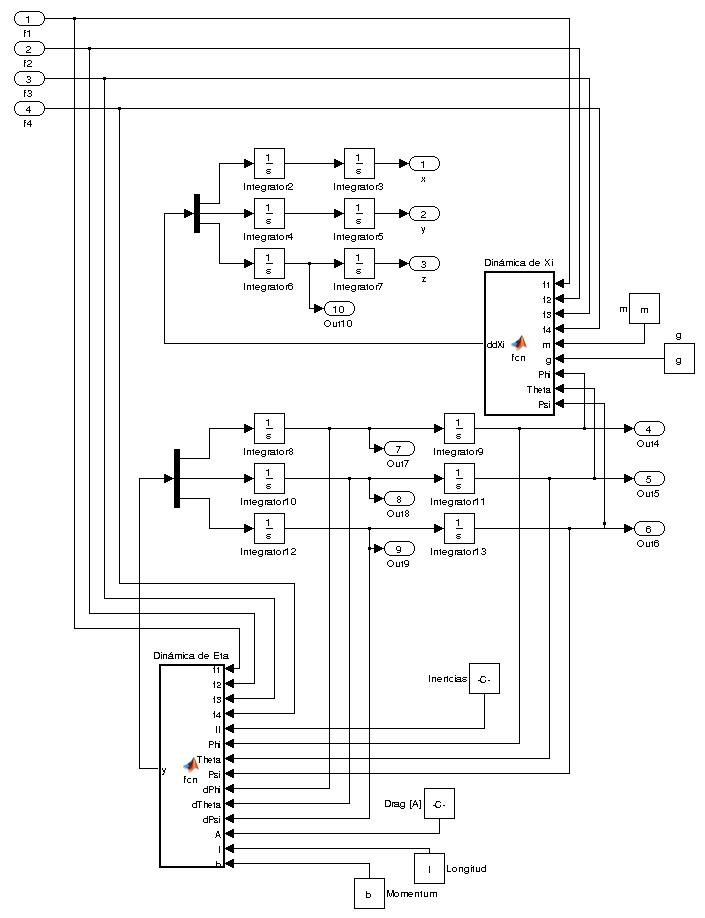
\includegraphics[scale=0.6]{images/Simulink_model.jpeg}
\caption{Modelo en Simulink de la dinámica del Quadcopter}
\end{center}
\end{figure}

Aunque en el modelo se hayan tenido en cuenta los respectivos coeficientes de fricción con el aire, como se ha visto en el apartado anterior no se han tenido en cuenta a la hora de linealizar el sistema ni calcular la ley de control ya que la determinación de estos parámetros no es fácil y de incluirse podría aportar incertidumbre. \\

Tal y como se explica a la hora de caracterizar los motores, no se pudo encontrar la relación existente que la fuerza y momento ejercido por cada hélice, por lo que en este caso se ha supuesto que varía proporcionalmente con $b$.

Los dos bloques presentes en el modelo ($Function \>\> Matlab$) definen su dinámica. La función $Dinámica \>\> de \>\> Xi$ determina las aceleraciones lineales. El código que se ejecuta en ésta es:\\


\begin{lstlisting}[language=Matlab]
function ddXi = fcn(f1,f2,f3,f4,m,g,Phi,Theta,Psi)
%#codegen

R=[[cos(Psi)*cos(Theta) cos(Psi)*sin(Theta)*sin(Phi)-sin(Psi)*cos(Phi) cos(Psi)*sin(Theta)*cos(Phi)+sin(Psi)*sin(Phi)];
   [sin(Psi)*cos(Theta) sin(Psi)*sin(Theta)*sin(Phi)+cos(Psi)*cos(Phi) sin(Psi)*sin(Theta)*cos(Phi)-cos(Psi)*sin(Phi)];
   [-sin(Theta) cos(Theta)*sin(Phi) cos(Theta)*cos(Phi)]];

T=[0; 0; (f1+f2+f3+f4)/m];

ddXi = R*T/m+[0; 0; -g];
\end{lstlisting}

En ella se calcula la matriz de rotación $\pmb{R}$ en función de la posición angular($\phi$,$\theta$ y $\psi$) y con el vector de fuerzas en la base móvil (del cuerpo $Body$) se calcula en vector de aceleraciones lineales, es decir, $\ddot{\xi}=\left[ \ddot{\phi} \quad \ddot{\theta} \quad \ddot{\psi} \right]^{T}$. \\

En la función $Dinámica \>\> de \>\> Eta$ se calculan las aceleraciones angulares. Su código corresponde a: 
\begin{lstlisting}[language=Matlab]
function y = fcn(f1,f2,f3,f4,II,Phi,Theta,Psi,dPhi,dTheta,dPsi,A,l,b)
%#codegen

Ixx=II(1);
Iyy=II(2);
Izz=II(3);
 
TauB=[[       l*(f4-f2)];
      [       l*(f3-f1)];
      [ b*(f1+f3-f2-f4)]];  

Weta=[[ 1         0         -sin(Theta)];
      [ 0  cos(Phi) cos(Theta)*sin(Phi)];
      [ 0 -sin(Phi) cos(Theta)*cos(Phi)]];
 
J=transpose(Weta)*[[Ixx 0 0];[0 Iyy 0];[0 0 Izz]]*Weta;  

CdE1=(Iyy*dTheta^2*sin(2*Phi))/2 - (Izz*dTheta^2*sin(2*Phi))/2 - Ixx*dPsi*dTheta*cos(Theta) - (Iyy*dPsi^2*sin(2*Phi)*cos(Theta)^2)/2 + (Izz*dPsi^2*sin(2*Phi)*cos(Theta)^2)/2 - Iyy*dPsi*dTheta*cos(2*Phi)*cos(Theta) + Izz*dPsi*dTheta*cos(2*Phi)*cos(Theta);

CdE2=dPhi*(Ixx*dPsi*cos(Theta) - 2*Iyy*dTheta*cos(Phi)*sin(Phi) + 2*Izz*dTheta*cos(Phi)*sin(Phi) + Iyy*dPsi*cos(Phi)^2*cos(Theta) - Izz*dPsi*cos(Phi)^2*cos(Theta) - Iyy*dPsi*cos(Theta)*sin(Phi)^2 + Izz*dPsi*cos(Theta)*sin(Phi)^2)  - Ixx*dPsi^2*cos(Theta)*sin(Theta) + Iyy*dPsi^2*cos(Theta)*sin(Phi)^2*sin(Theta)  + Izz*dPsi^2*cos(Phi)^2*cos(Theta)*sin(Theta);

CdE3=-dPhi*(Ixx*dTheta*cos(Theta) - Iyy*dTheta*cos(Phi)^2*cos(Theta) + Izz*dTheta*cos(Phi)^2*cos(Theta) + Iyy*dTheta*cos(Theta)*sin(Phi)^2 - Izz*dTheta*cos(Theta)*sin(Phi)^2 - 2*Iyy*dPsi*cos(Phi)*cos(Theta)^2*sin(Phi) + 2*Izz*dPsi*cos(Phi)*cos(Theta)^2*sin(Phi))  - Iyy*dTheta^2*cos(Phi)*sin(Phi)*sin(Theta) + Izz*dTheta^2*cos(Phi)*sin(Phi)*sin(Theta) + 2*Ixx*dPsi*dTheta*cos(Theta)*sin(Theta) - 2*Izz*dPsi*dTheta*cos(Phi)^2*cos(Theta)*sin(Theta) - 2*Iyy*dPsi*dTheta*cos(Theta)*sin(Phi)^2*sin(Theta);

CdEta=[CdE1; CdE2; CdE3];

y = inv(J)*(TauB-CdEta);
\end{lstlisting}
En esta función se calcula el vector de momentos ($\pmb{TauB}$), se calcula la actual matriz de cambio de base de velocidad angular a derivadas de ángulos de Euler ($\pmb{W_\eta}$), se actualiza el tensor de inercias según este cambio y se obtiene el producto $\pmb{C(\eta,\dot{\eta})}\cdot\pmb{\dot{\eta}}$. Finalmente devuelve las aceleraciones según se obtienen en la ecuación \ref{eq:system2}.

Los parámetros que se cargan en Matlab necesarios para definir este modelo son
\begin{lstlisting}[language=Matlab]
% Declaracion simbolica de las variables

syms x dx ddx y dy ddy z dz ddz Phi dPhi ddPhi Theta dTheta ddTheta Psi dPsi ddPsi
syms f1 f2 f3 f4 
syms Ixx Iyy Izz
syms Ax Ay Az 
syms k m g l b

l=0.165					% Longitud de los brazos
Ixx=0.004				% Producto de inercia en x
Iyy=0.004				% Producto de inercia en y
Izz=0.008				% Producto de inercia en z
m=0.85					% Masa del Quadcopter
b=1.2*10^-7				% Relacion Momento-Fuerza
g=9.81					% Aceleracion gravedad

Ax=0					% Friccion aire (no usado)
Ay=0
Az=0
\end{lstlisting}


\newpage
\section{Diseño del controlador} \label{control}

Con el modelo linealizado del sistema ya se tiene lo que emulará una respuesta verosímil y acorde a la realidad.Para que haga lo que uno espera  se decide aplicar un control óptimo mediante un regulador LQR (Linear Quadratic Regulator). \\

\subsection{Regulador Quadrático Lineal}
% Explicar teoría del regulador

Dado un sistema lineal de tiempo continuo definido por 

\begin{equation}
\begin{array}{l}
\pmb{\dot{X}}=[\pmb{A}] \cdot \pmb{X} + [\pmb{B}] \cdot \pmb{U} \\
\pmb{Y} = [\pmb{C}] \cdot \pmb{X} 
\end{array}
\end{equation} 

se quiere operar este sistema mediante un coste mínimo según un criterio determinado. Este criterio se caracteriza por tener una función de costes $\mathbf{J}$ que depende tanto de los estados como de las entradas del sistemas \cite{LQR_Wikipedia}

\begin{equation}
\mathbf{J} =\int^{\infty}_{0} \left( \pmb{X^{T}}\mathbf{Q}\pmb{X} + \pmb{U^{T}}\mathbf{R}\pmb{U} + 2\pmb{X^{T}}\mathbf{N}\pmb{U} \right) dt
\end{equation}

y se definen los pesos $\mathbf{Q}$, $\mathbf{R}$ y $\mathbf{N}$ como matrices definidas positivas y simétricas, según la penalización que se le quiera dar a los estados ($\mathbf{X}$), acciones ($\mathbf{U}$) o el efecto de ambos ($\mathbf{N}$)respectivamente, tal que se minimice el coste $\mathbf{J}$. Se obtiene la ley de control $\pmb{U}=-\pmb{K} \cdot \pmb{X}$ de 
\begin{equation}
\pmb{K}=\mathbf{R}^{-1} \left( \pmb{B}^{T} \mathbf{S} + \mathbf{N}^{T} \right) 
\end{equation}

donde $\mathbf{S}$ es la solución de la ecuación de Riccati asociada 

\begin{equation}
\pmb{A}^{T}\mathbf{S} + \mathbf{S}\pmb{A} - \left( \mathbf{S}\pmb{B}+\mathbf{N} \right) \mathbf{R}^{-1} \left( \pmb{B}^{T} \mathbf{S} + \mathbf{N}^{T} \right) + \mathbf{Q} = - \dot{\mathbf{S}}
\end{equation}

En este caso se supondrá que $\mathbf{N}=0$ (ver \cite{LQR_Matlab}) se tendrá

\begin{equation}
\mathbf{J} =\int^{\infty}_{0} \left( \pmb{X^{T}}\mathbf{Q}\pmb{X} + \pmb{U^{T}}\mathbf{R}\pmb{U} \right) dt
\end{equation}

y por consiguiente, la ecuación a resolver es

\begin{equation}
\pmb{A}^{T}\mathbf{S} + \mathbf{S}\pmb{A} - \mathbf{S}\pmb{B} \mathbf{R}^{-1} \pmb{B}^{T} \mathbf{S} + \mathbf{Q} = 0
\end{equation}

Finalmente, de éste procedimiento se obtiene, además de las constantes de realimentación $\pmb{K}$ y la solución $\pmb{S}$, los polos del sistema: $\pmb{P}=eig( \pmb{A} - \pmb{B} \cdot \pmb{K})$.


\subsection{Obtención de la ley de control}
% Cálculo de las k's

Como se ha visto en la ecuación \ref{eq:final_system}, las matrices que representan el sistema son

\begin{equation}
\pmb{A}= \left[ \begin{array}{cccc}
0 & 1 & 0 & 0 \\
0 & 0 & 0 & 0 \\
0 & 0 & 0 & 1 \\
0 & 0 & 0 & 0 \\ \end{array} \right] \hspace{1cm} \pmb{B}=\left[ \begin{array}{cccc}
0 & 0 & 0 & 0 \\
0 & {}^{-l}/_{Ixx} & 0 & {}^{l}/_{Ixx} \\ 
0 & 0 & 0 & 0 \\
{}^{-l}/_{Iyy} & 0 & {}^{l}/_{Iyy} & 0 \\ \end{array} \right] 
\end{equation} 

\begin{equation}
\nonumber
\pmb{C}=\left[ \begin{array}{cccc}
1 & 0 & 0 & 0 \\
0 & 0 & 1 & 0 \\ \end{array} \right] 
\end{equation} 

En el apartado anterior se ha visto que se deben asignar valores a $\mathbf{Q}$ y $\mathbf{R}$, y como tanto $\mathbf{X}$ como $\mathbf{U}$ son vectores $4x1$, las matrices a asignar serán $4x4$. La matriz $\mathbf{Q}$ se puede escribir como 

\begin{equation}
\mathbf{Q}=1 \cdot \pmb{C}^{T}\pmb{C}
\end{equation}

por lo tanto 

\begin{equation}
\mathbf{Q}= \left[ \begin{array}{cc}
1 & 0 \\
0 & 0 \\
0 & 1 \\
0 & 0 \\ \end{array} \right] \left[ \begin{array}{cccc}
1 & 0 & 0 & 0 \\
0 & 0 & 1 & 0 \\ \end{array} \right] = \left[ \begin{array}{cccc}
1 & 0 & 0 & 0 \\
0 & 0 & 0 & 0 \\
0 & 0 & 1 & 0 \\
0 & 0 & 0 & 0 \\ \end{array} \right]
\end{equation}

Para el caso de $\mathbf{R}$ se consideran toda un mismo peso para todas las entradas $f_i$ y muy superior a los pesos de $\mathbf{Q}$: 

\begin{equation}
\mathbf{R}=100 \cdot I = \left[ \begin{array}{cccc}
100 &   0 &   0 &   0 \\
0   & 100 &   0 &   0 \\
0   &   0 & 100 &   0 \\
0   &   0 &   0 & 100 \\ \end{array} \right] 
\end{equation}

Se hayan $\mathbf{K}$,$\mathbf{S}$ y $ \mathbf{E}$ mediante la toolbox de Matlab para calcular el control óptimo según el regulador LQR\cite{Toolbox_lqr}:

\begin{verbatim}
            [K,S,e] = LQR(A,B,Q,R)
\end{verbatim}

Teniendo en cuenta que los parámetros del sistema físico obtenidos en el Anexo 4 son $Ixx=...$, $Iyy=...$ y $l=...$ se tiene que:

\begin{equation}
\mathbf{K}= ... \hspace{2cm} \mathbf{S}=... 
\end{equation}
\begin{equation}
\nonumber
\mathbf{E}=...
\end{equation}

\subsection{Aplicación en el modelo}


\newpage
\section{Implementación del control} \label{implement}
% Pufff

\newpage
\section{Construcción del Quadcopter} \label{construc}
% Descripción de cómo se hará en general
El conjunto de piezas que forman este aparato están conectadas entre sí según la función que realicen. Esencialmente la Raspberry Pi controla los motores según les señales que recibe de la IMU y el Receptor. Todo el conjunto es alimentado por una batería LiPo y se adapta el voltaje de 11.1V a 5V por medio de un Regulador para poder alimentar a la Raspberry. Todos los componentes están sujetos a una estructura (Frame) que también subre las fuerzas y momentos.  

\subsection{Descripción de los componentes}
% Descripción y explicación de cada componente del Quadcopter, con imágenes de cada
Se describe seguidamente cada componente y el criterio de selección que se ha aplicado.
\subsubsection*{Raspberry Pi} 
Abreviado com a RPi, es un pequeño ordenador integrado en una sola placa (Single-Board Computer o SBC en inglés) del tamaño de una tarjeta de crédito, es dir, con unas dimensiones de 85.6cm x 53.98cm, desarrollada por la Fundación Raspberry Pi con la intención de promocionar las ciencias computacionales en las escuelas \cite{RPiWiki}. 

%\begin{tabular}{cc}
\begin{figure}[h!]
\begin{center}
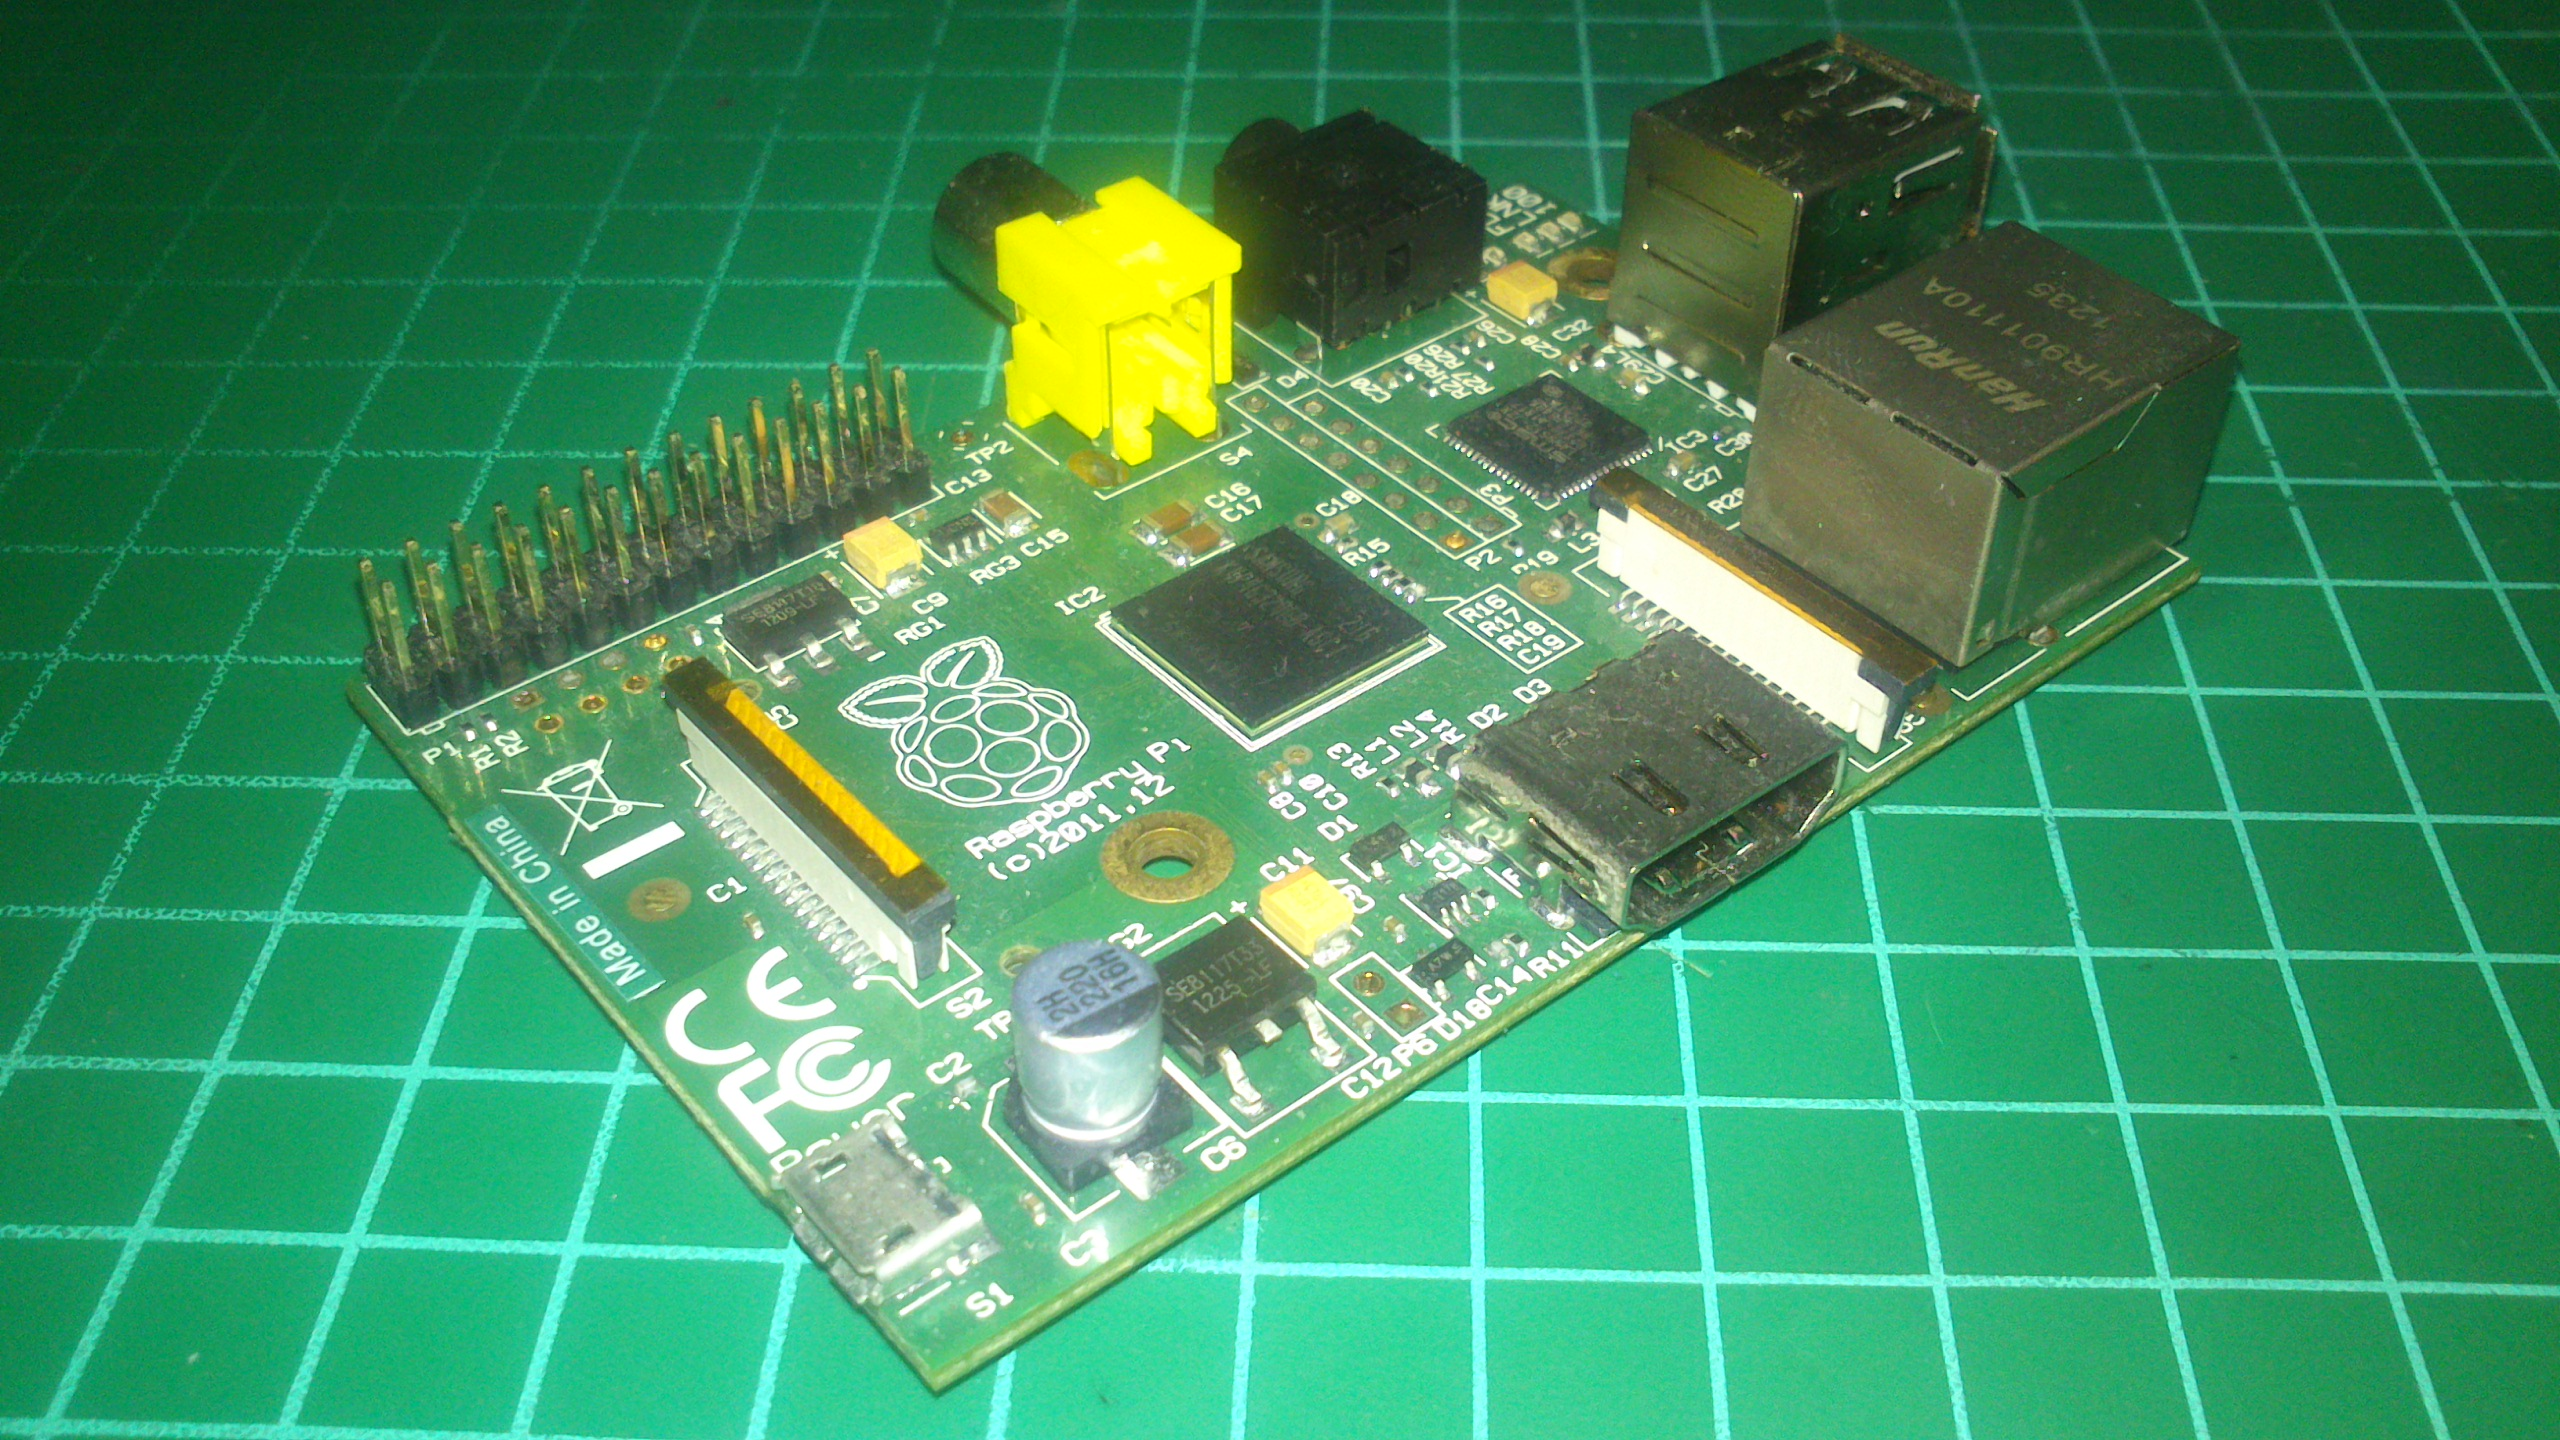
\includegraphics[scale=0.06]{images/RPi.jpg}
\caption{Raspberry Pi a utilizar}
\label{RPiImage}
\end{center}
\end{figure}
%\end{tabular}

Se ha optado por esta opción por su económico precio, la velocidad de procesamiento y bajo consumo. Además, se han querido ampliar los conocimientos de este pequeño monstruo. En particular se utiliza la segunda revisión del modelo B:

\begin{figure}[h!]
\begin{center}
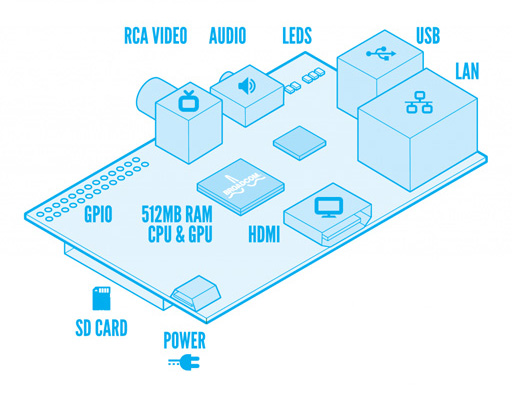
\includegraphics[scale=0.3]{images/RPi2.jpg}
\caption{Conectores de la Raspberry Pi}
\label{RPiConn}
\end{center}
\end{figure}

%\begin{tabular}{cc}
%\hspace{1cm}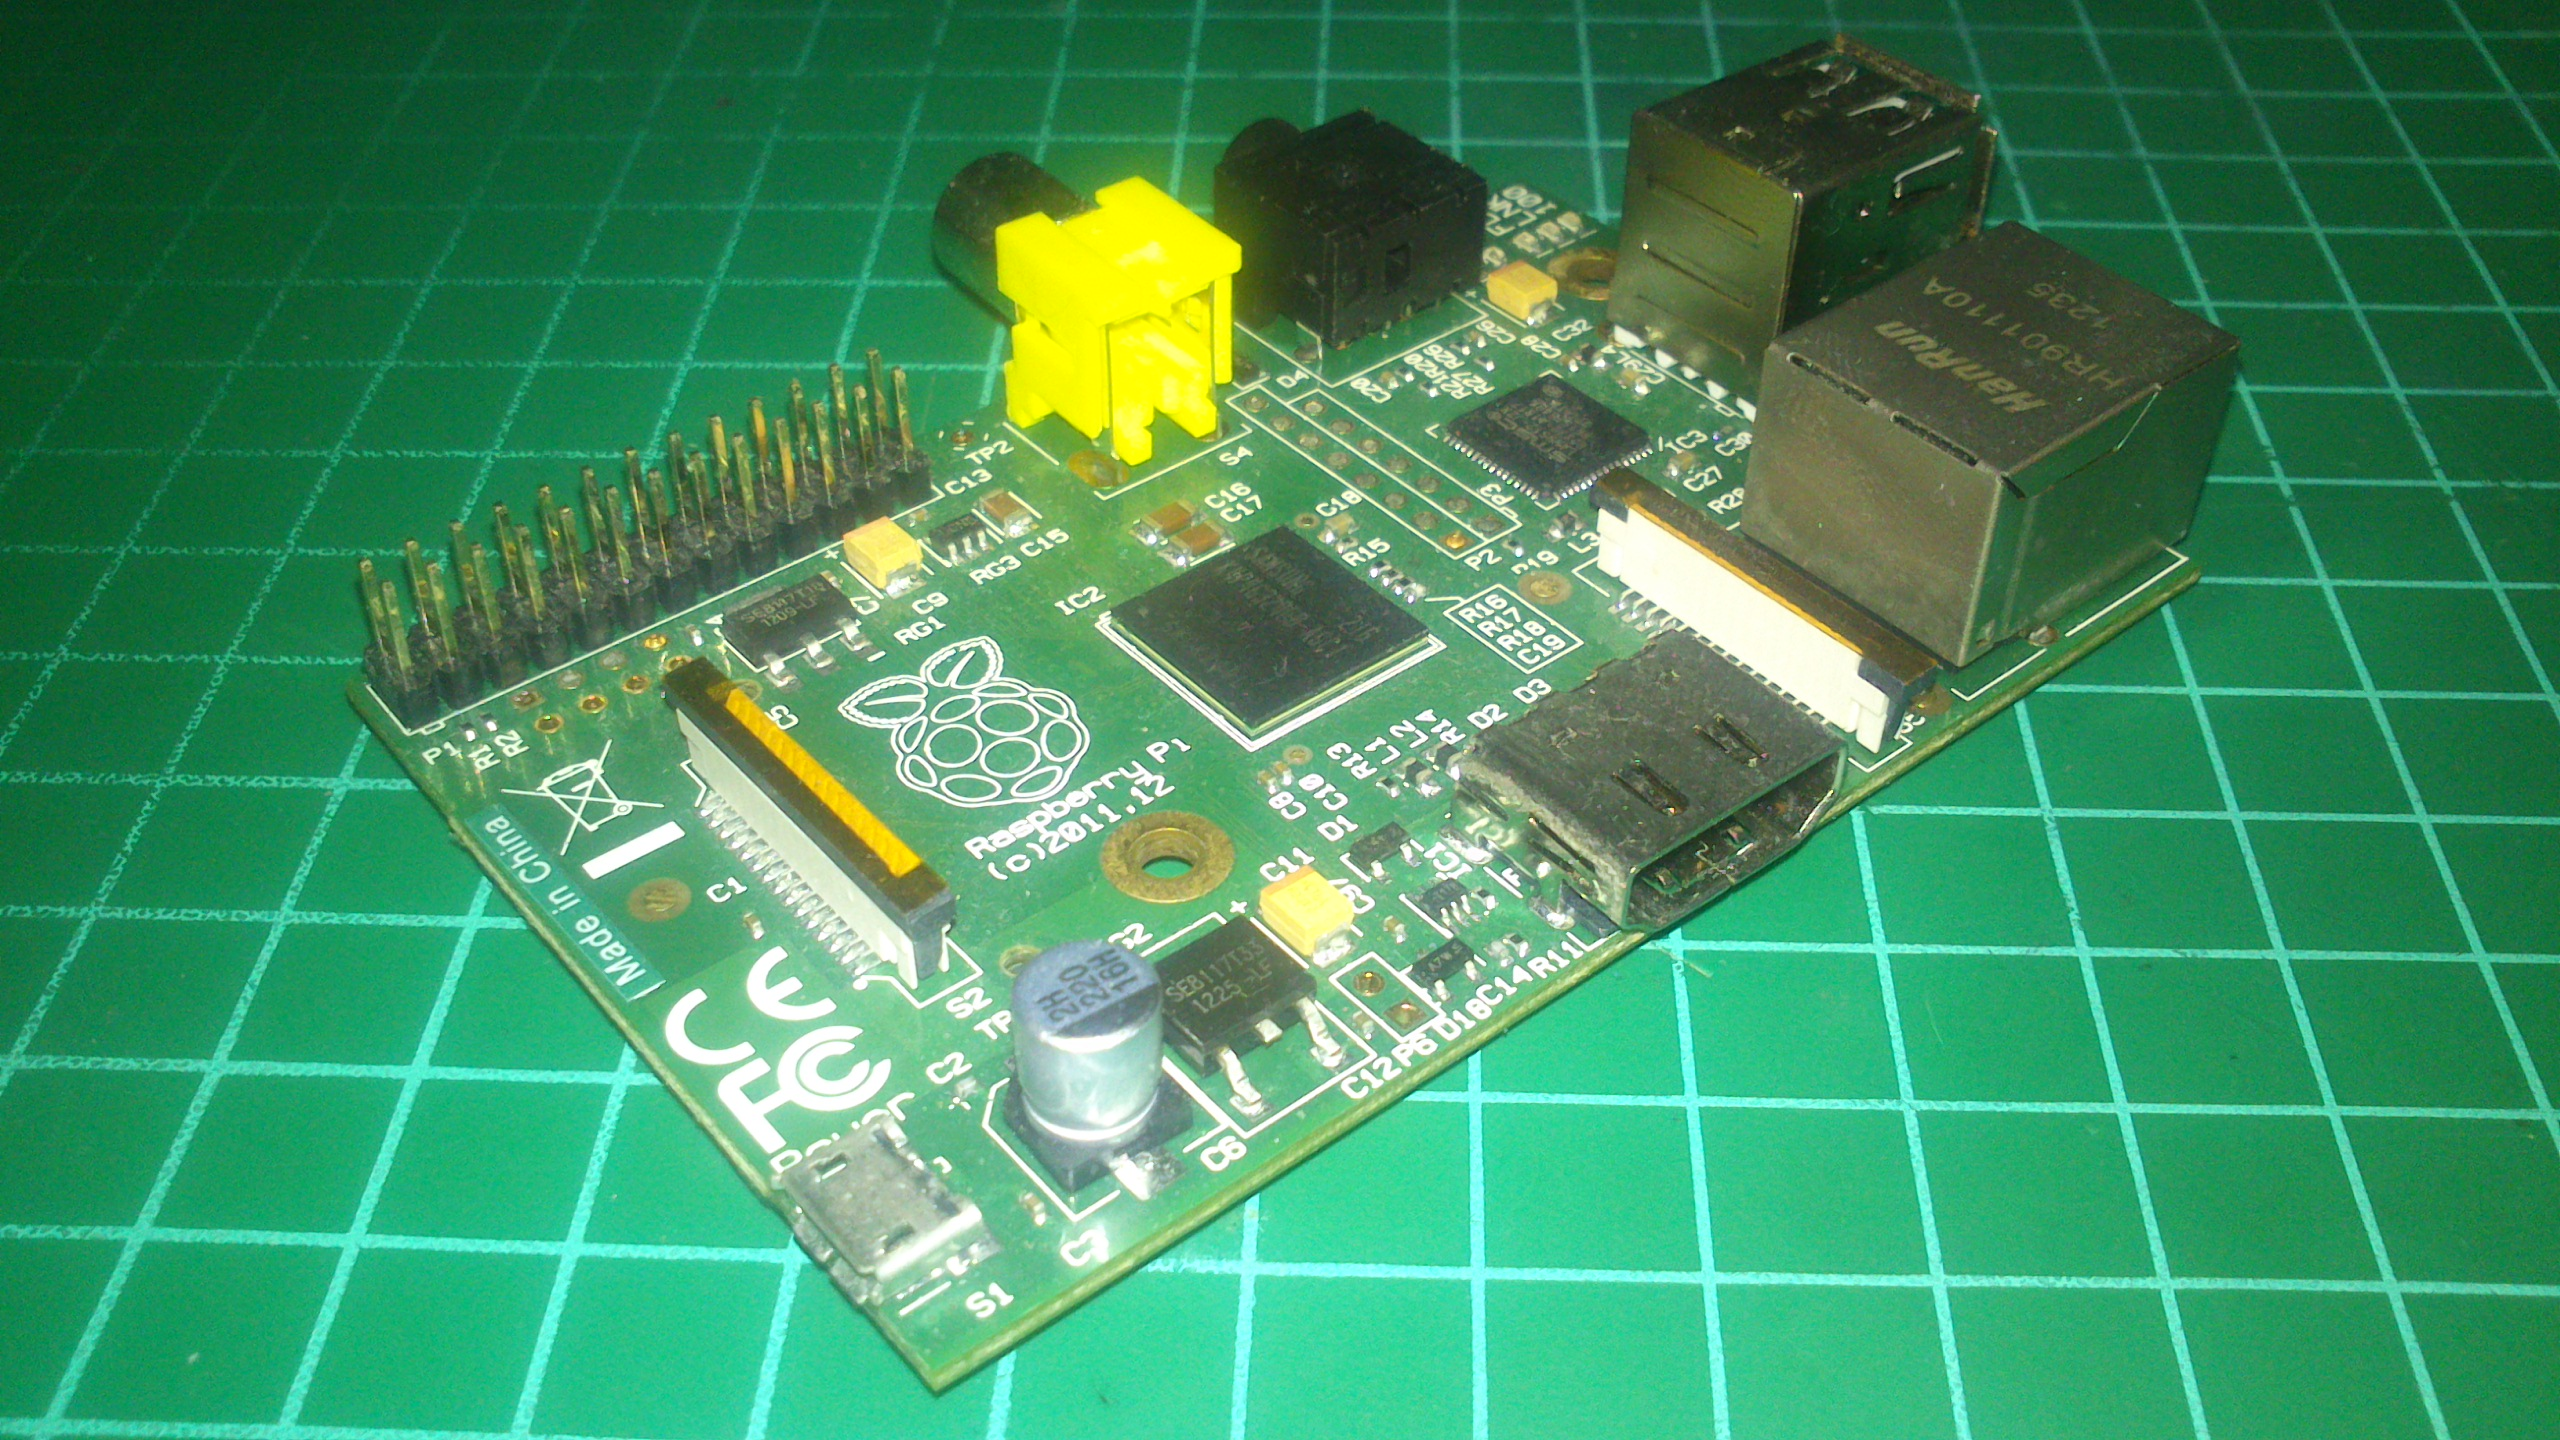
\includegraphics[scale=0.06]{images/RPi.jpg}
%& \hspace{0.5cm} 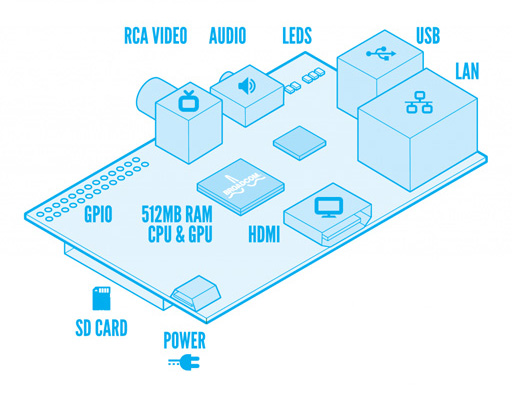
\includegraphics[scale=0.3]{images/RPi2.jpg}
%\end{tabular} \\

Tiene un System-on-Chip (SoC) Broadcom BCM2835 con un ARM1176JZF-S a 700 Mhz, una GPU VideoCore IV y 512 MB de memoria RAM. Dispone de dos puertos USB, una salida mini-jack 3.5mm, salida de audio/vídeo HDMI, una salida RCA y un puerto  RJ45 10/100 de Ethernet. 

La alimentación se realiza por medio de un mini USB a 5V/700mA, con un consumo de 3.5W. El sistema operativi es un Raspbian, grabado en una tarjeta SD de 4GB. Dispone de un conjunto de pines que permiten comunicación con periféricos de bajo nivel UART, I2C, SPI y 8 pines de propósito general (General Porpouse Input Output o GPIO).

\subsubsection*{GY-521 MPU-6050} 
Se trata de una Unidad de Medida Inercial (IMU en inglés) que integra en un mismo encapsulado de $4x4x0.9mm$ un acelerómetro y un giróscopo, ambos de 3 ejes. Dispone de un conversor ADC de 16 bits para cada eje y se comunica mediante un protocolo de comunicación $I2C$. Se ha optado por utilizar este dispositivo por su bajo coste y la fácil implicada con la RPi.
\begin{figure}[h!]
\begin{center}
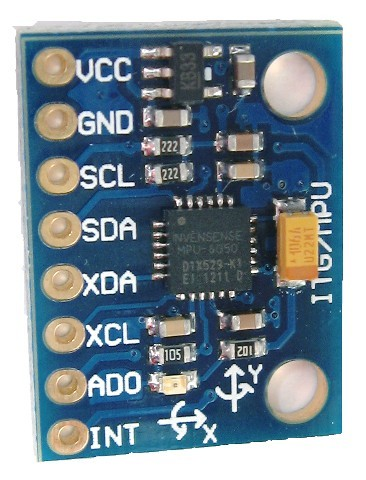
\includegraphics[scale=0.12]{images/mpu-6050.jpg} 
\caption{IMU MPU-6050}
\end{center}
\end{figure}\\
Como características de los sensores: el giróscopo tiene un rango de  $\pm250,\pm500,\pm1000,\pm2000$ grados/segundo, y el acel·lerómetro de $\pm2g,\pm4g,\pm8g,16g$. La tensión de alimentación es del rango de $2.375V-3.46V$ y cabe la posibilidad de utilizar un módulo $DMP$ (Digital Motion Processor), pero se ha decidido implementar un filtro de Kalman para leer los datos en crudo (raw) de la cola $FIFO$ del sensor.

\subsubsection*{Emisor-Receptor}
Con este aparato de se transmite la consigna generada des del transmisor hacia el receptor mediante ondas de radio. El modelo que se utiliza es el $Turnigy 5X 5Ch Mini$, porque es fácil de utilizar y además económico. Las especificaciones técnicas más relevantes son: 

\begin{figure}[h!]
\begin{center}
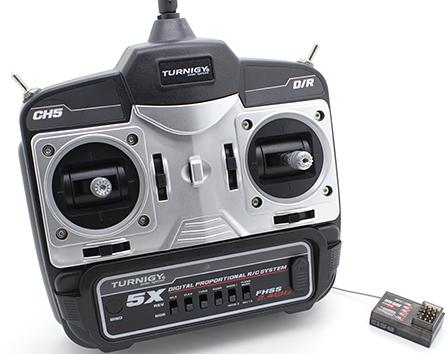
\includegraphics[scale=0.4]{images/E_R.jpg} 
\caption{Emisora y Receptor}
\end{center}
\end{figure}

El transmisor tiene unas dimensiones de $156x152x50mm$, un peso de 265g y se alimenta a 6V (4 baterías AA). El receptor tiene unas medidas de $33.5x20.5x13mm$ y se alimenta a 4.8-6V. Dispone de 5 canales de radio, con transmisión segura a 2.4GHz con el método FHSS. Puede configurarse para trabajar con dos modos(mode1-mode2).

La señal que se recibe para cada canal en el receptor es de $PWM$ de $50Hz$ con un Duty que varía de $1ms$ a $2ms$.

%% Especificación por canal de los PWM: mínimo y máximo Duty
%% Mirar con osciloscopio la señal

\subsubsection*{Batería LiPo}
Para alimentar a todo el conjunto se utiliza una LiPo $Turnigy 2200mAh 3S1P 25C$. Por tanto, es capaz de entregar 2.2A durante una hora, y como la capacidad es de 25C, la descarga puede ser de $2.2*25=55A$ con un pic de descarga de 35C, es dir, con un pico de $2.2*35=77A$ durante 10 segundos. Esta batería está formada por tres celdas que proporcionan un voltaje total de unos $11.1V$:\\

\begin{figure}[h!]
\begin{center}
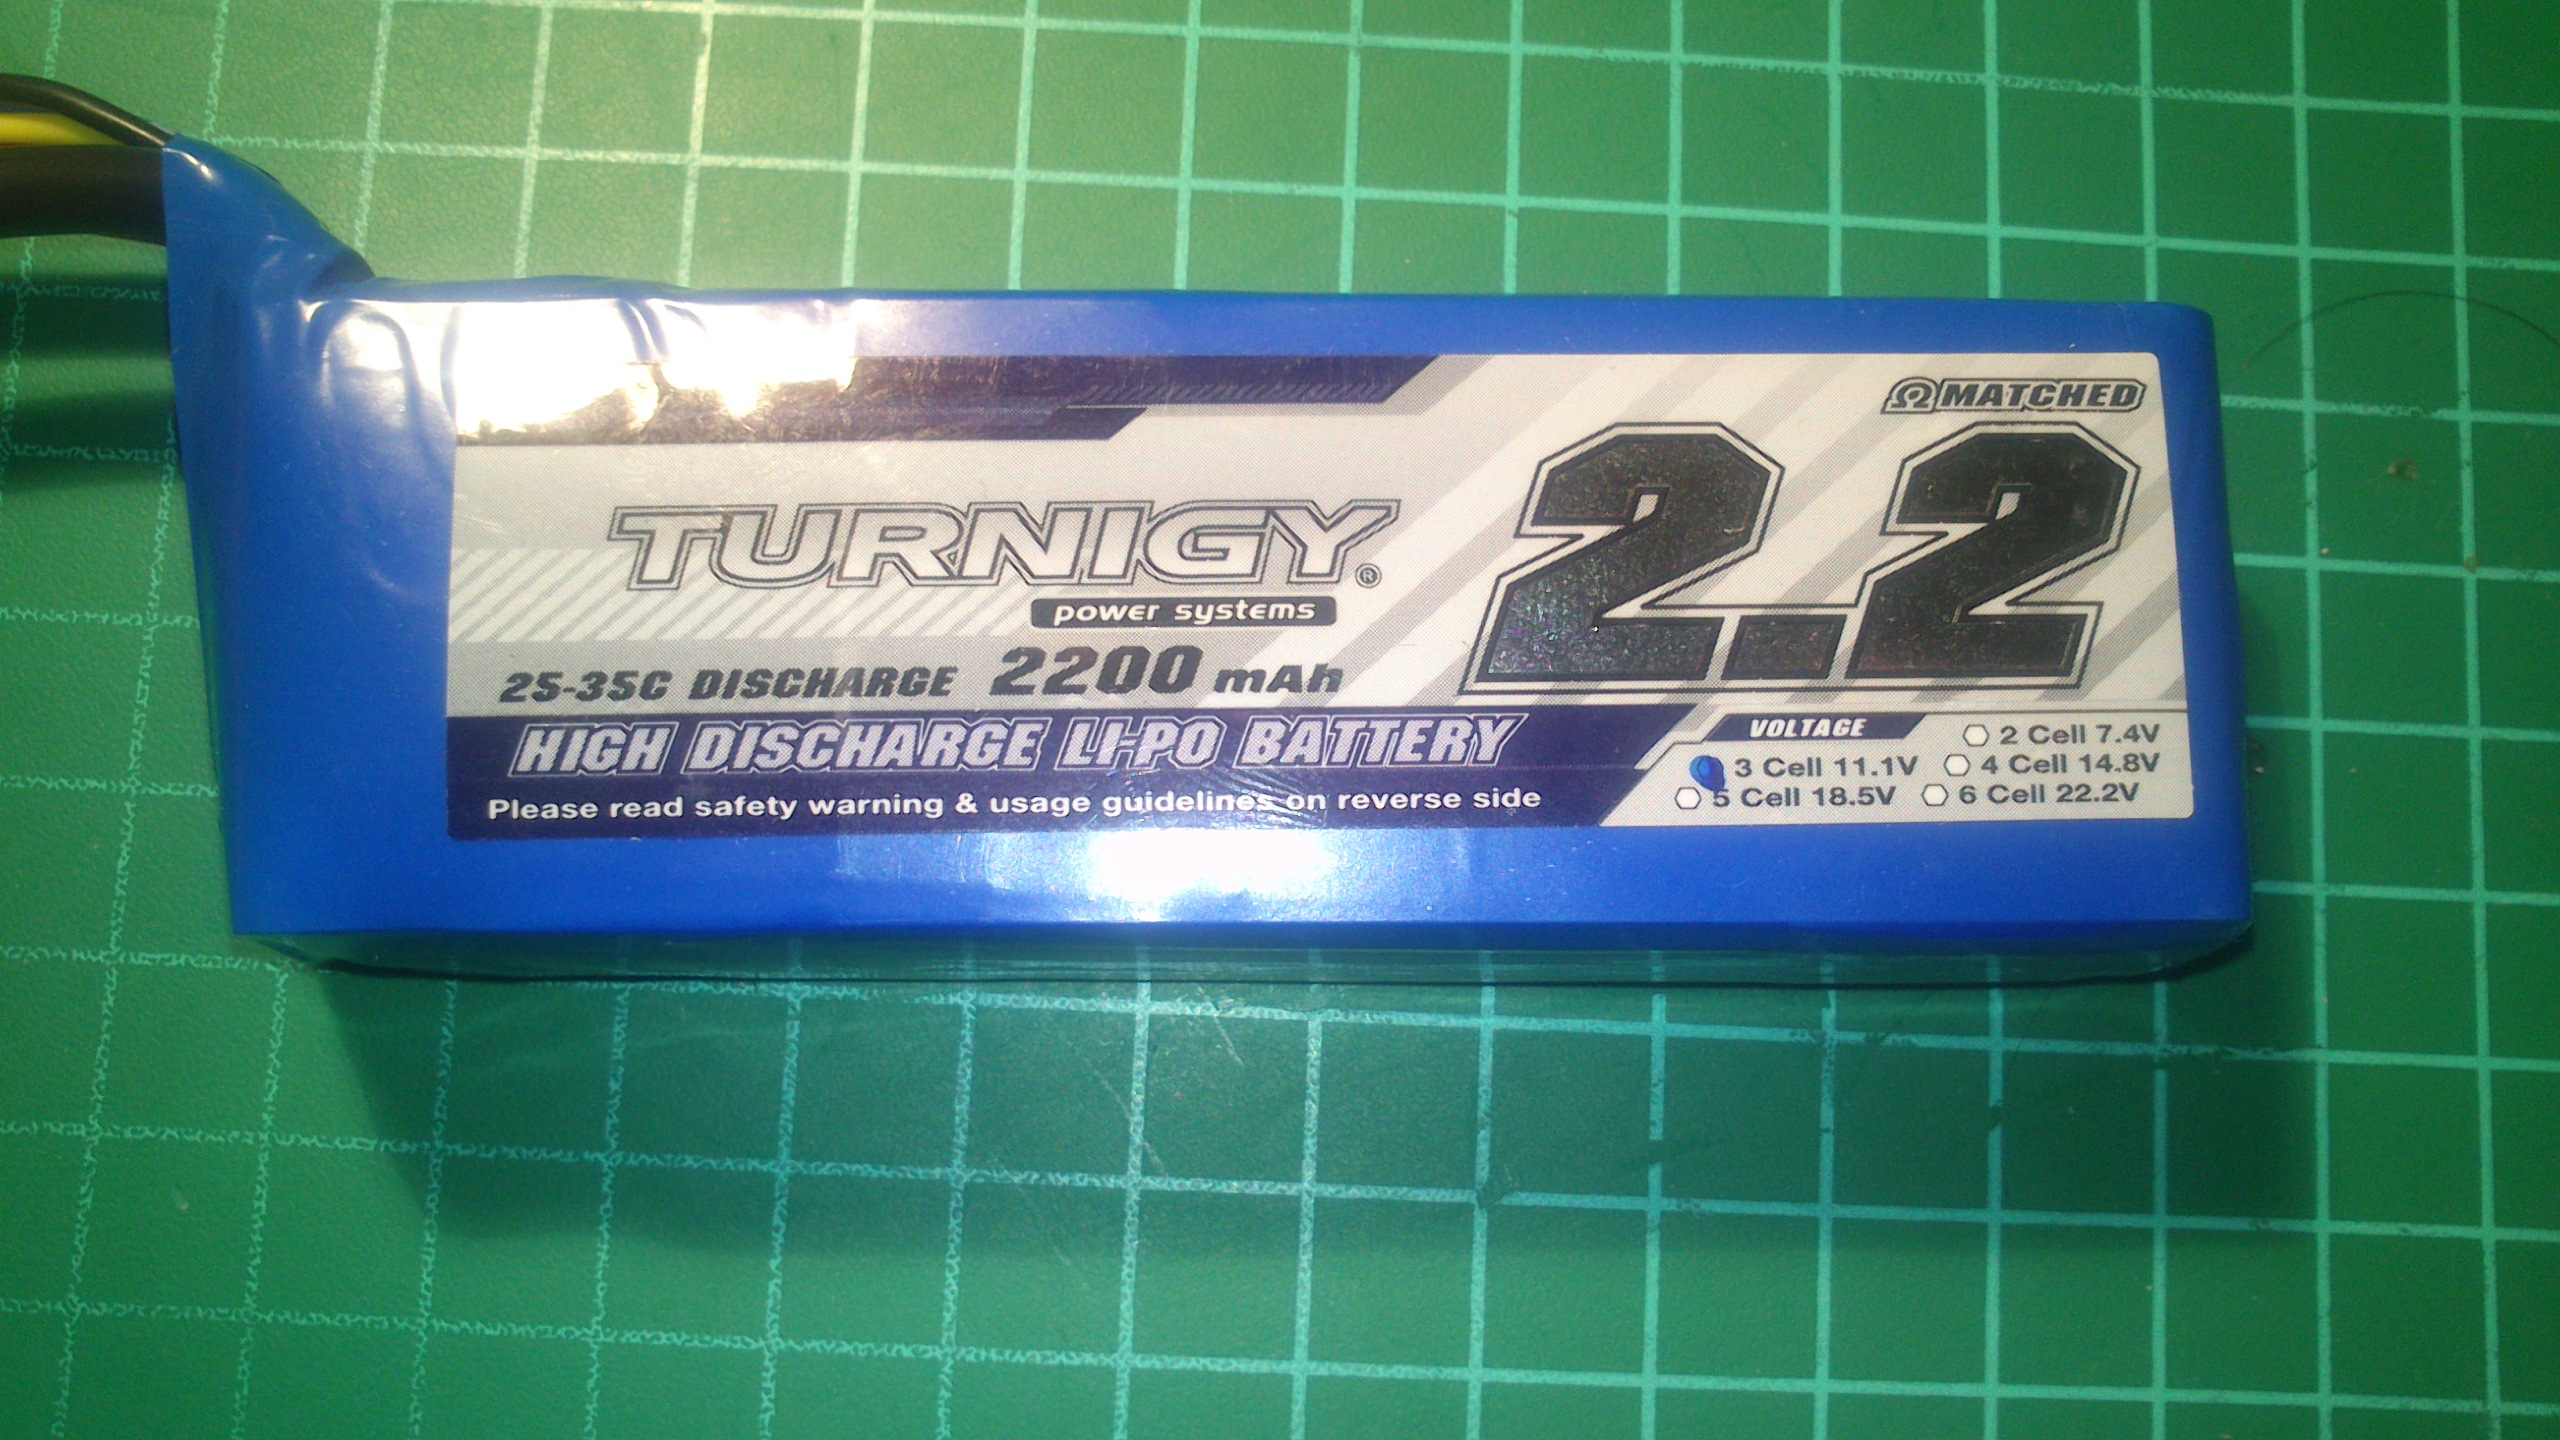
\includegraphics[scale=0.1,viewport=0 400 2560 1250,clip]{images/LiPo.jpg} \\
\caption{Batería LiPo empleada}
\end{center}
\end{figure}

El conector de carga es el $JST-XH$ y el de descarga el $XT60$. Para tener en cuenta respecto al Quadcopter es interesante saber que pesa $188g$ y respecto a la estructura (frame) que sus dimensiones son de $105x33x24mm$.

\subsubsection*{Regulador Step-Down}
Para adaptar la tensión de 11.1V de la batería LiPo a 5V para alimentar la Raspberry Pi, es necesario un regulador. En este caso se tiene el Interruptor-Modo Máximo BEC LM2576S, que proporciona hasta 3A de corriente \\

\begin{figure}[h!]
\begin{center}
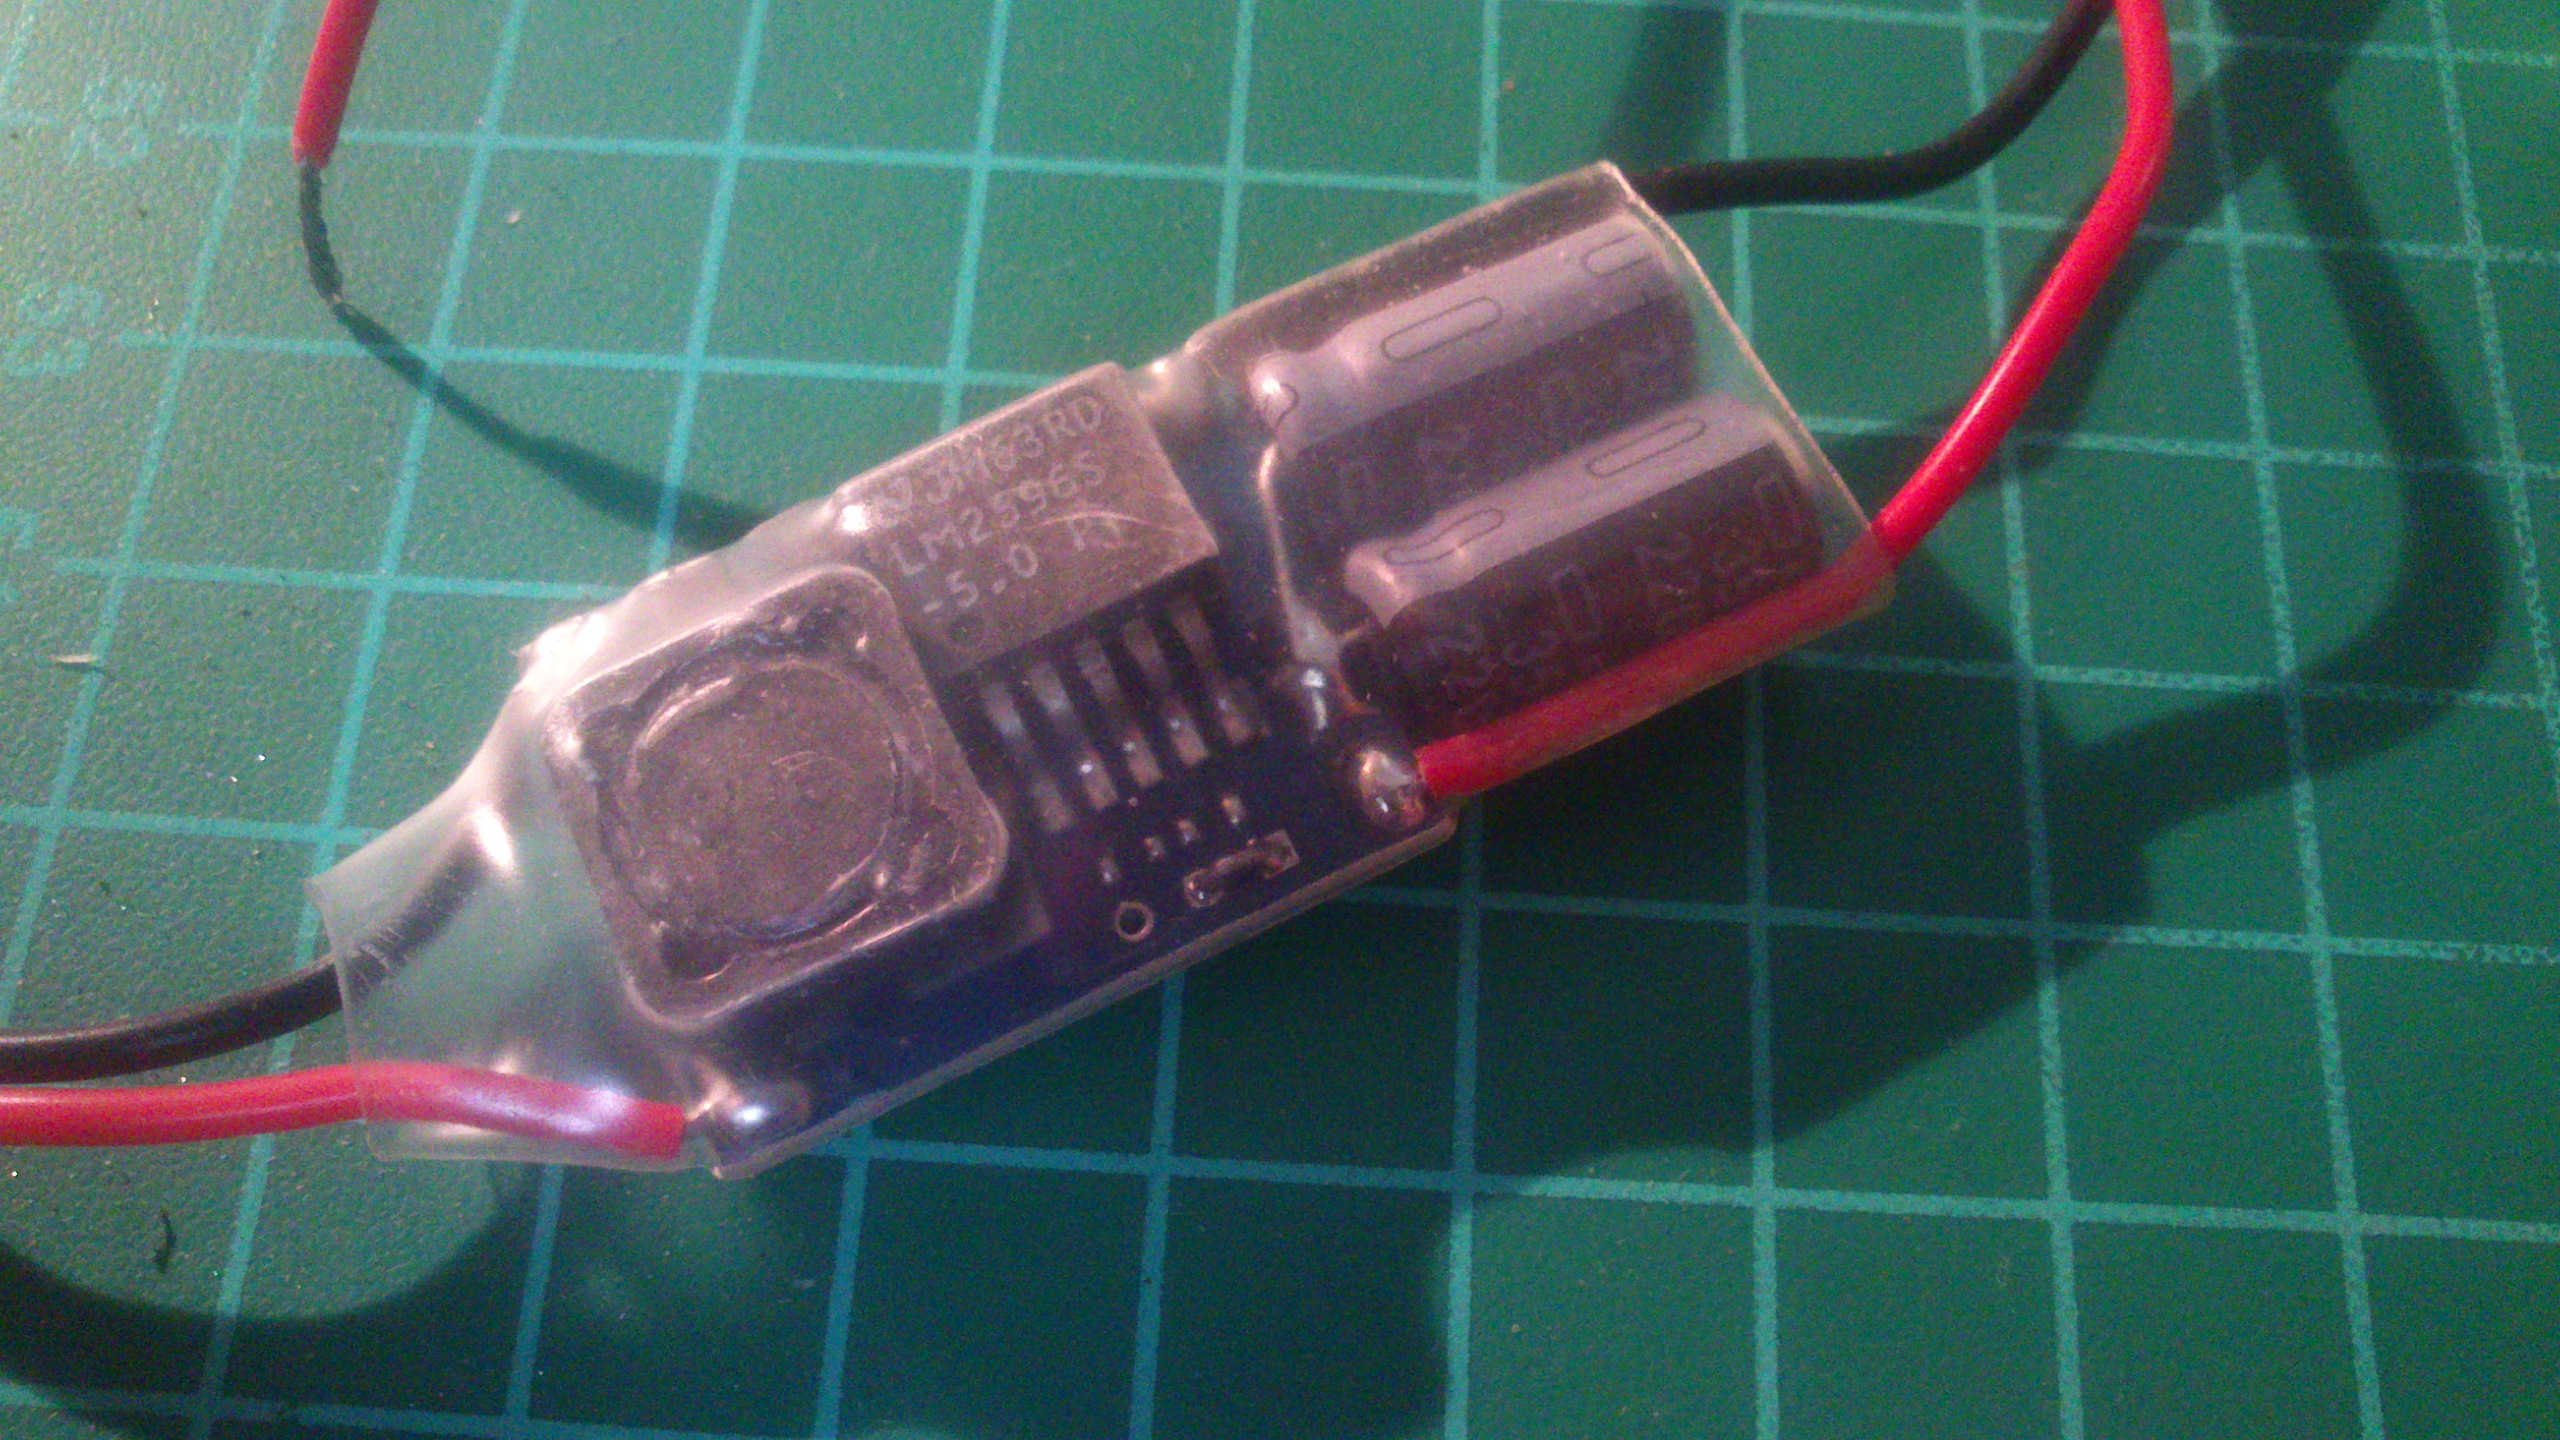
\includegraphics[scale=0.06]{images/Reg_stepdown.jpg}
\caption{Regulador Step-Down}
\end{center}
\end{figure}

El esquema del componente \cite{lm2576s}:

\begin{figure}[h!]
\begin{center}
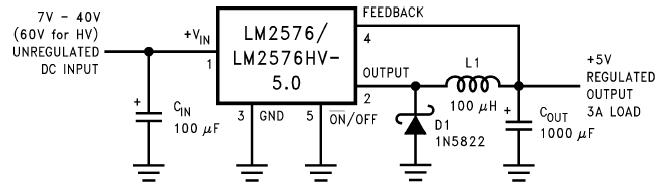
\includegraphics[scale=0.55]{images/lm2576s.jpeg} 
\caption{Esquema del Regulador Step-Down}
\end{center}
\end{figure}


\subsubsection*{Motores Brushless}
Los actuadores que se utilizan son motores brushless (BL-DC). En particular el Turnigy 2213 20turn 1050kv 19A Outrunner.
Se trata de máquinas síncronas de imanes permanentes, en vez de utilizar electroimanes, donde el campo magnético está uniformemente repartido  en el entrehierro. Se conocen también de fuerza electromotriz (FEM) trapezoidal porque a velocidad constante la FEM tiene esta forma. 
Para controlarlo se utiliza un inversor (inverter), y como la conmutación deja de ser mecánica la armadura de la máquina puede ser el estátor. Ésto permite llegar a voltajes de uso y velocidades de funcionamiento más altas.
Sus especificaciones más relevantes son:
\begin{itemize}
\item Kv: 1050rpm/V
\item Corriente de trabajo: 6A ~ 16A
\item Corriente de pico: 19A
\item Peso: 56g
\item Dimensiones: 27.6 x 32mm
\item Medida de el eje: 3.175mm
\end{itemize}

El primer parámetro hace referencia a cuántas rpm's funcionará el motor por Voltio aplicado. A este valor se le aplica un porcentaje $\%NLS$ (Porcentaje de Velocidad sin Carga, típicamente de 70\%) para saber cuántas revoluciones por minuto funcionará:

\begin{equation}
Kv  \cdot V \cdot \%NLS = 1050 \cdot \frac{rpm}{V}\cdot V \cdot 0.70 = 8085 \>\> rpm
\end{equation}

Esta velocidad es teórica, y como que no hay un lazo de control sobre ésta, no se tendrá en cuenta. En cambio, se atacará al motor con la señal de PWM que se envía al Variador que le controla. La relación entre la señal de PWM y la fuerza, así como el consumo que se desarrolla se encuenta en los Anexos. 

\subsubsection*{Variador ESC}


Para controlar un motor brushless la etapa de potencia a utilitzar es un ESC (Electronic Speed Controller) que es un  variador que se compone de un inversor trifásico:
\begin{figure}[h!]
\begin{center}
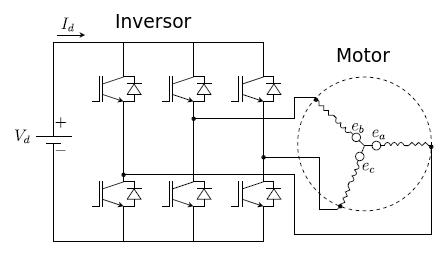
\includegraphics[scale=0.4]{images/ESC.jpeg}
\caption{Esquema de un Variador como inversor trifásico}
\end{center}
\end{figure}
El modelo a utilitzar es el Turnigy AE-20A Brushless ESC. El uso de este tipo se justifica con el amperaje que soporta, en cuanto los motores consumen un pico de hasta 19A, que es menor al màximo de la corrente de este Variador (como límite se puede quemar el componente si se hacen circular 25A durante 10 segundos). 
Se debe asegurar la compatibilidad con la batería también, ya que soporta tensiones de entrada correspondientes a Baterías LiPo de entre 2 y 4 celdas. 
Incluye un circuito BEC (Battery Eliminator Circuit) para poder alimentar también el receptor de 2A de máxima corriente. 
La máxima velocidad de funcionamiento del motor depende de sus polos: si es de 2 polos será de 210000 rpm, con 6 polos de 70000 rpm y de 12 polos a 35000 rpm.


Tanto el peso de $19$g,  como las dimensiones de $50x26x12$mm son parámetros a tener en cuenta en el montaje, en parte a que se hubican en los brazos del Quadcopter, aumentando la inercia por eje e influyendo considerablemente en el modelo. Antes de usar cada Variador se ha tenido que programar para que éste responda con un mejor rendimiento al caso en cuestión.

\begin{figure}[h!]
\begin{center}
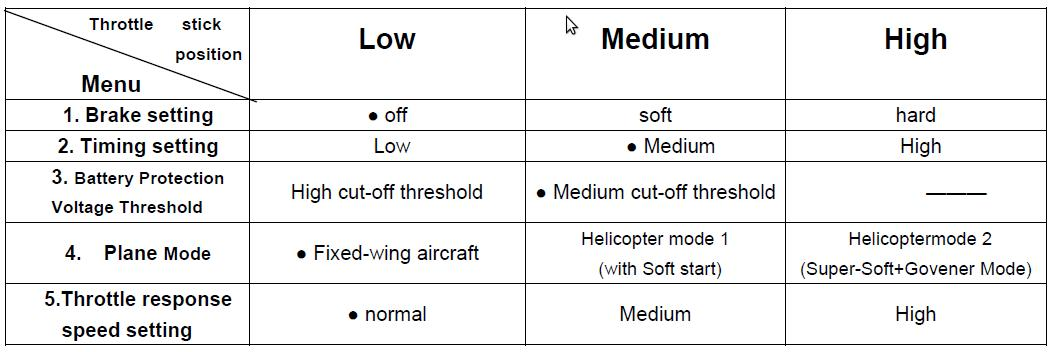
\includegraphics[scale=0.45]{images/ESC_config.jpeg}
\caption{Tabla de Set up de un ESC}
\end{center}
\end{figure}

Para los 5 parámetros a configurar hay tres opciones, y las marcadas con un punto son las que se han aplicado.

\subsubsection*{Marco}

Todos los elementos que componen el Quadcopter se sujetan en una estructura que mantiene la integridad y rigidez necesarias para el vuelo.

\begin{figure}[h!]
\begin{center}
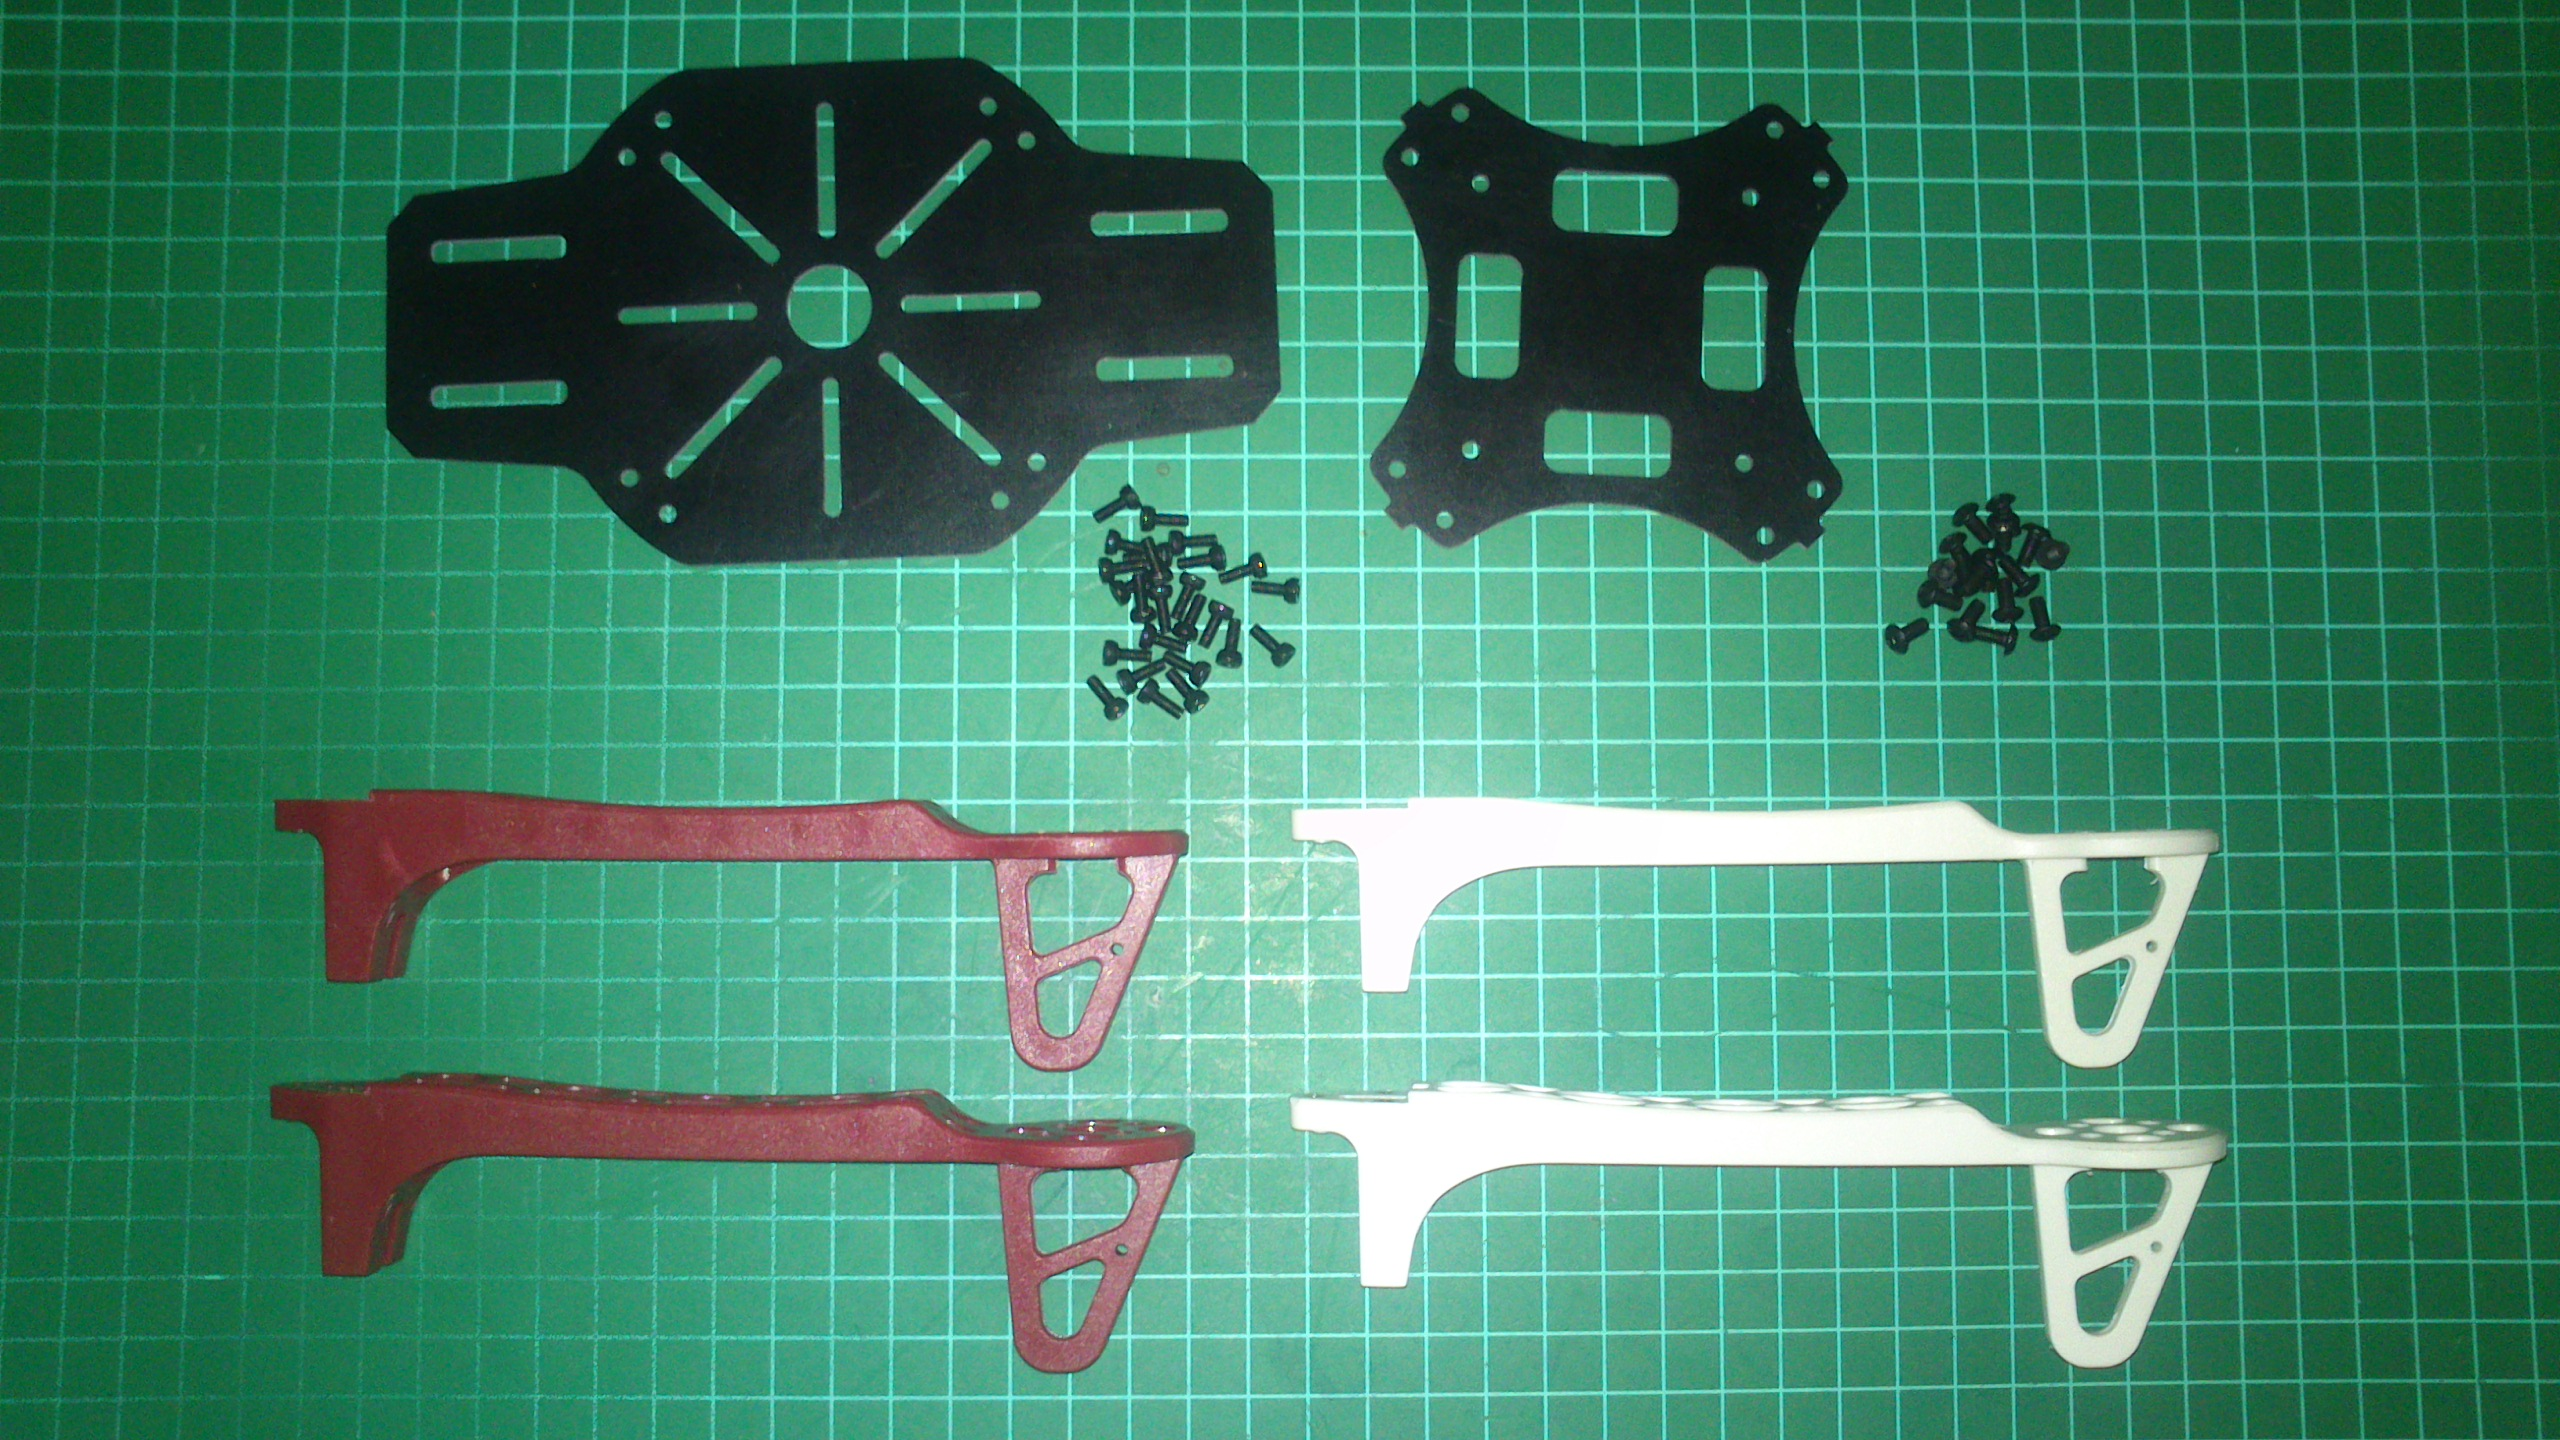
\includegraphics[scale=0.1]{images/frame.jpg}
\caption{Piezas que componen la estructura del Quadcopter}
\end{center}
\end{figure}

La mayor parte del peso se concentra en el centro de la estructura e interesa que sea lo más ligera posible sin comprometer su integridad, de tal manera que los motores, situados en las puntas de cada brazo, deban compensar el menor peso posible. En este caso, tiene un peso de 190g, y las piezas están hechas de fibra de vidrio las piezas centrales (de color negro en la imagen) y de Nylon los brazos (rojo y blanco en la imagen). La distancia entre dos motores de una diagonal es de 33cm.


\subsubsection*{Hélices}

En girar el motor, las aspas solidarias a su eje utilizan la energía cinética del rotor para proporcionar sustentación propulsando aire en sentido contrario. El tipo de aspa condiciona el rendimiento que se obtenga, así que se utilizan las que optimizan la fuerza de propulsión respecto al consumo de corriente. El modelo de hélice utilizado es el 8x4

\begin{figure}[h!]
\begin{center}
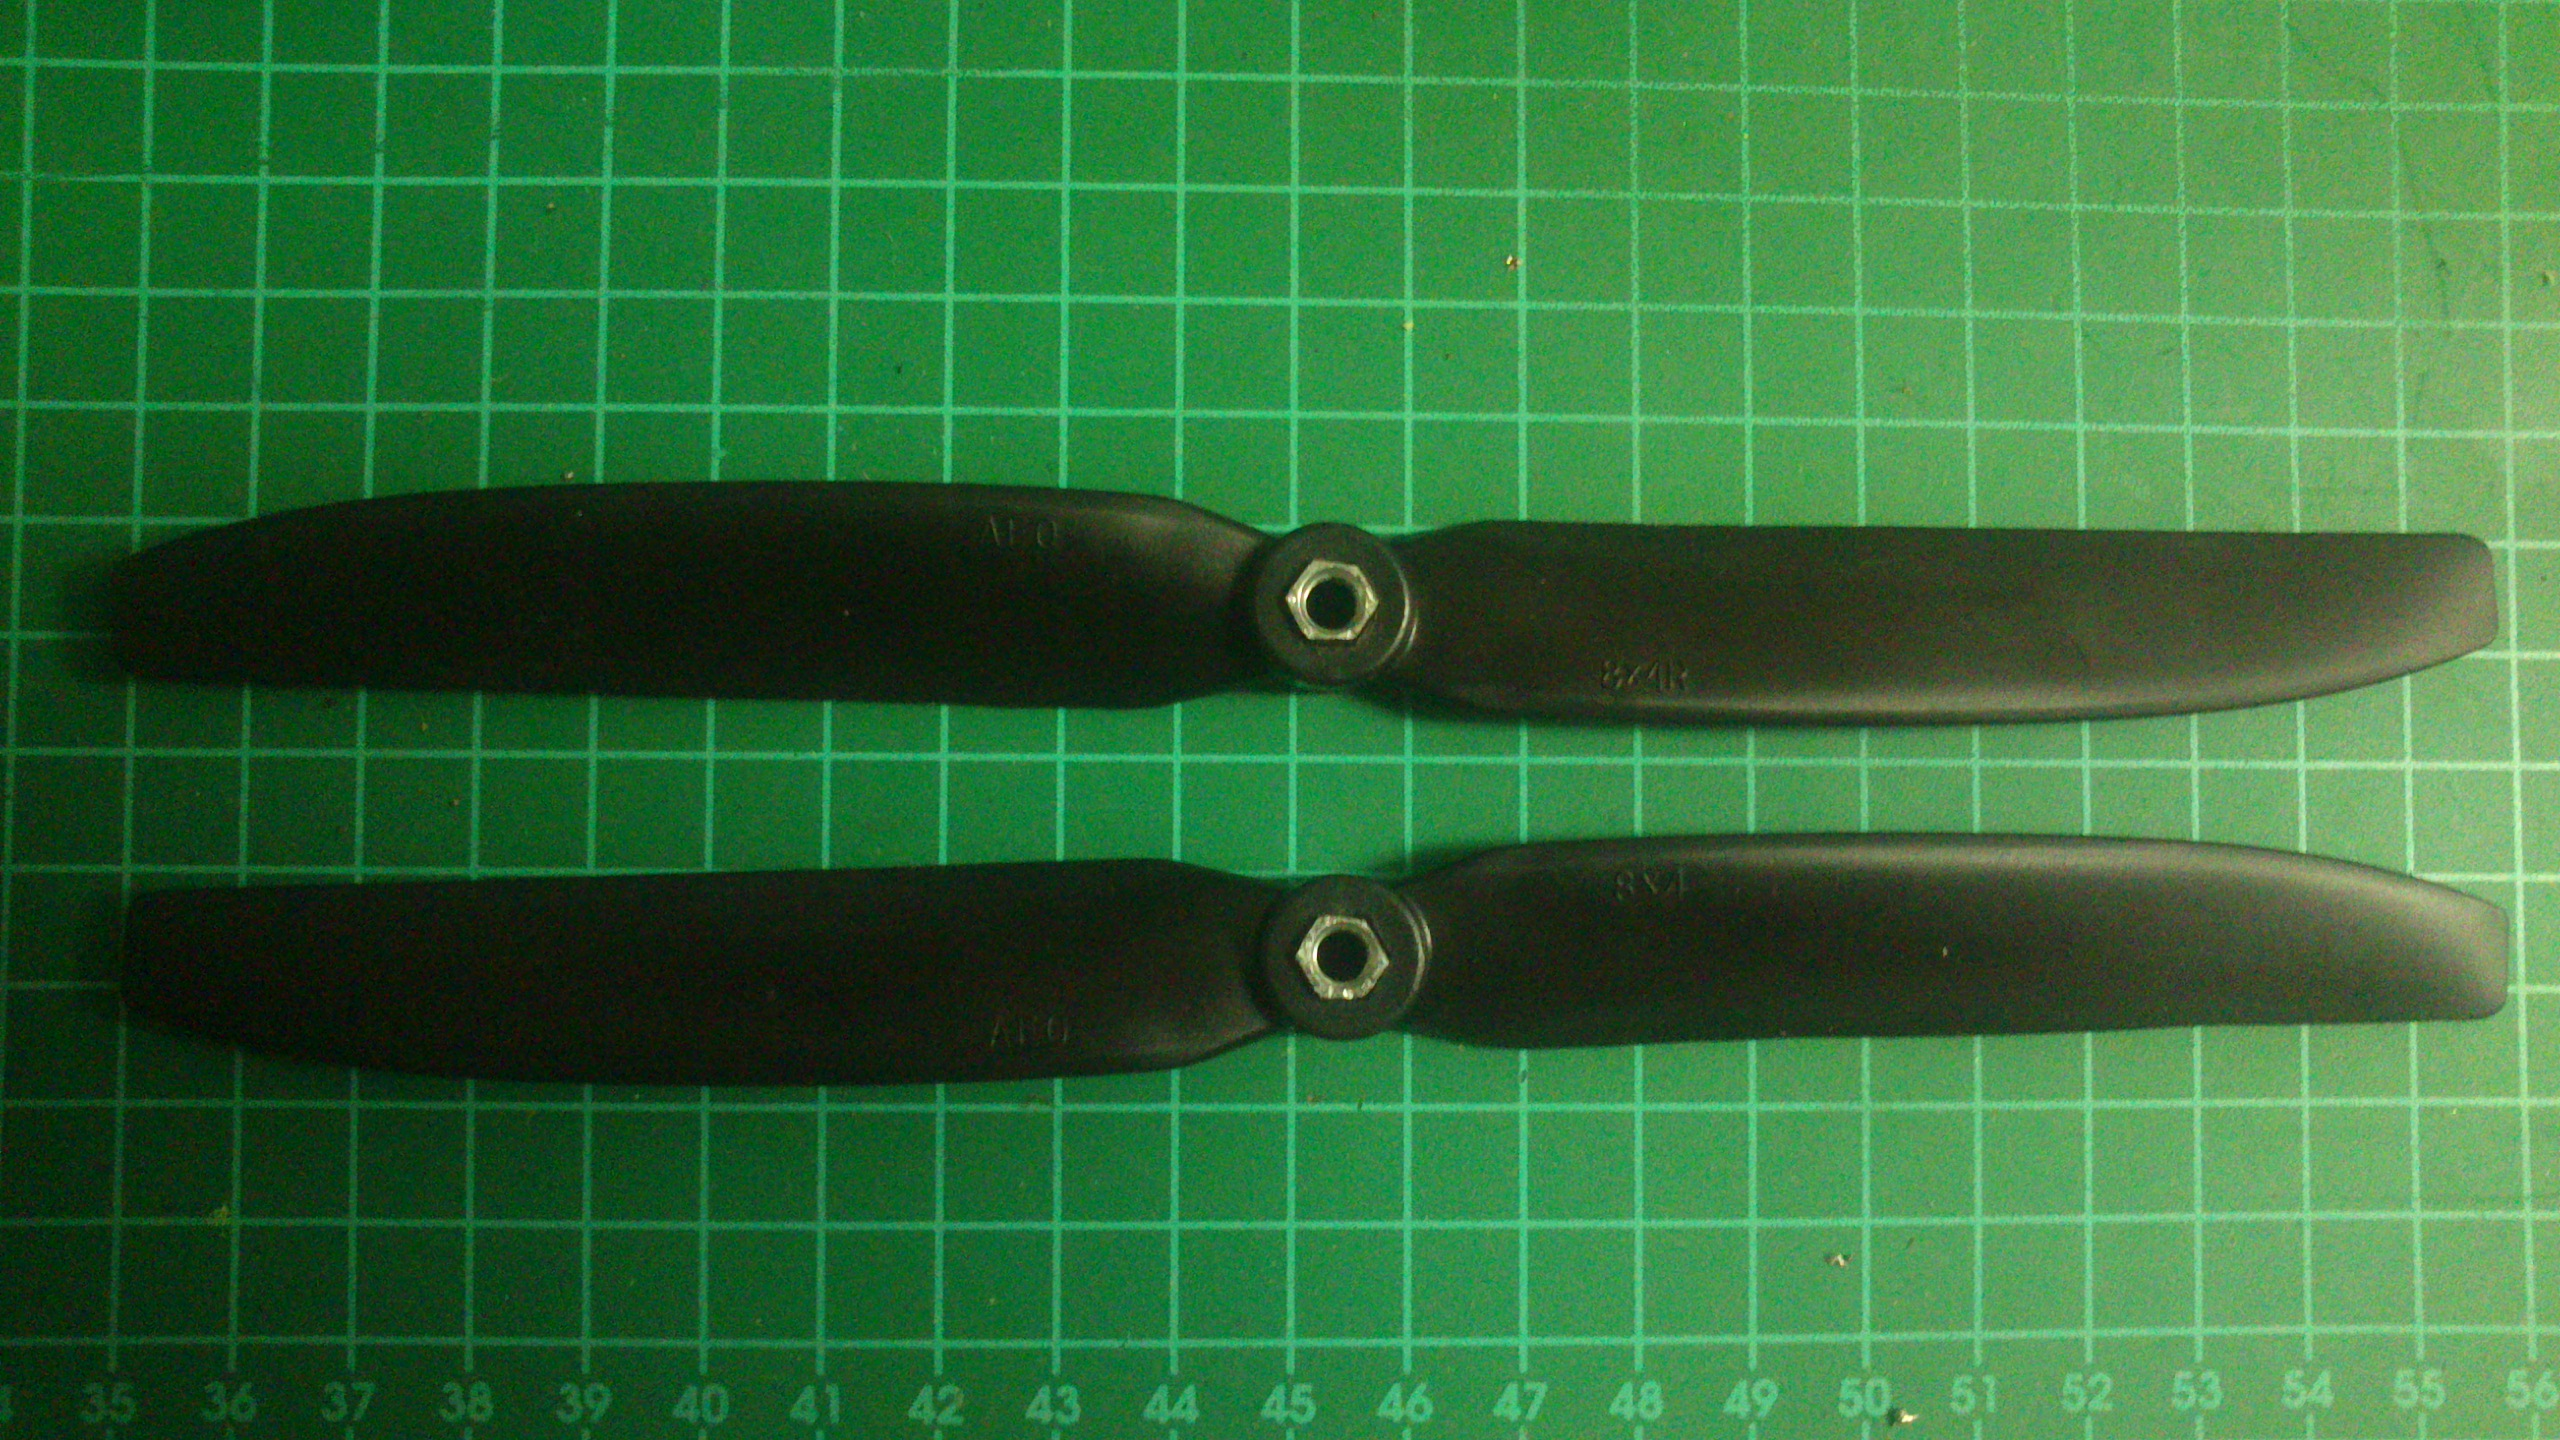
\includegraphics[scale=0.065,viewport=0 200 2560 1100,clip]{images/propeller_image.jpg}
\caption{Par de hélices 8x4 simétricas}
\end{center}
\end{figure}

Los parámetros que definen una hélice son su Longitud ($X$), és decir, diámetro de superficie recorrida por las aspas en pulgadas, y el Pitch ($Y$), que es la distancia que se avanzaría la hélice en una revolución de moverse en una masa blanda. Se representan en el siguiente gráfico:

\begin{figure}[h!]
\begin{center}
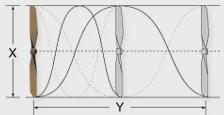
\includegraphics[scale=0.9]{images/propeller_xy.jpeg}
\caption{Representación de la Longitud y Pitch de una Hélice}
\end{center}
\end{figure} 

\newpage
\subsection{Montaje}
% Descripción del procedimiento por pasos y con fotos

\begin{center}
\begin{tikzpicture}
%%% POWER LINES
\path[draw] (1,8.25) node {\large 12V};
\path[draw] (2,8.25) node {\large 0V};
\path[draw,line width=6pt,color=red,o-o] (1,1) -- (1,8);
\path[draw,line width=6pt,color=black,o-o] (2,1) -- (2,8);

%%% LIPO LEVEL
\path[draw,line width=2pt,color=red] (1,6) -- (3,6);
\path[draw,line width=2pt,color=black] (2,5.5) -- (3,5.5);
\path[draw] (3.8,5.75) node[draw,line width=3pt] (nodeA) {\huge LiPo};
\path[draw] (7.2, 5.75) node[draw,line width=3pt] (nodeA) {\huge IMU};
\path[draw,line width=2pt,color=olive] (7.2,5.35) -- (7.2,4.6);
\path[draw] (7.6,5) node (nodeC) { I2C};
\path[draw] (9.8, 5.75) node[draw,line width=3pt] (nodeA) {\huge Rec.};
\path[draw, line width=2pt,color=green] (9.8, 5.34) -- (9.8, 4.5) -- (7.95, 4.5);
\path[draw] (9, 4.8) node {5xCHNL};
\path[draw,line width=2pt,dotted, color=cyan](10.6,5.75) -- (12.3,5.75);
\path[draw] (13, 5.75) node[draw,line width=3pt] (nodeA) {\huge Em.};

%%% BUCK LEVEL
\path[draw,line width=2pt,color=red] (1,4.5) -- (3,4.5);
\path[draw,line width=2pt,color=black] (2,4) -- (3,4);
\path[draw] (4.1,4.25) node[draw,line width=3pt] (nodeA) {\huge BUCK};
\path[draw,line width=2pt,color=red] (5.26,4.5) -- (6.5,4.5);
\path[draw,line width=2pt,color=black] (5.2,4) -- (6.5,4);
\path[draw] (7.2,4.25) node[draw,line width=3pt] (nodeA) {\huge RPi};
\path[draw] (5.8,4.8) node (nodeC) {5V};
\path[draw, line width=2pt, color=green] (7.95,4)--(9.8,4) -- (9.8,3.2);
\path[draw] (9.2,3.65) node {PWM};

%%% ESC LEVEL
\path[draw, line width=2pt, color=red] (1,3) -- (9,3);
\path[draw, line width=2pt, color=black] (2,2.5) -- (9,2.5);
\path[draw] (9.8,2.75) node[draw,line width=3pt] (nodeC) {\huge ESC};
\path[draw] (10.3,2.1) node (nodeC) {\large (x4)};
\path[draw, line width=2pt, color=blue] (10.6,3) -- (12,3);
\path[draw, line width=2pt, color=blue] (10.6,2.75) -- (12,2.75);
\path[draw, line width=2pt, color=blue] (10.6,2.5) -- (12,2.5);
\path[draw] (13,2.75) node[draw,line width=3pt] (nodeC) {\huge Motor};
\path[draw] (13.7,2.1) node (nodeC) {\large (x4)};
\end{tikzpicture}
\end{center}

\newpage

\section{Análisis económico} \label{economics}

\newpage

\section{Estudio del impacto ambiental} \label{impacto}

\newpage

\section{Conclusiones} \label{conclusiones}

\subsection*{Futuras aplicaciones}

\newpage

\begin{thebibliography}{99}
\bibitem{QuadPaper} Teppo Luukkonen (August 22,2011). \textit{Modelling and control of quadcopter}
\bibitem{RPiWiki} Wikipedia de la Raspberry Pi: \url{http://en.wikipedia.org/wiki/Raspberry_Pi}
\bibitem{IMUArduino} Acelerómetro y giroscopio MPU-6050 para Arduino: \url{http://playground.arduino.cc/Main/MPU-6050#.UzhsVCK9jb4}
\bibitem{6050Esp} MPU-6050. Especificación del producto: \url{http://www.invensense.com/mems/gyro/documents/PS-MPU-6000A-00v3.4.pdf}
\bibitem{6050RegMap} MPU-6050. Mapa de Registros y descripciones: \url{http://www.invensense.com/mems/gyro/documents/RM-MPU-6000A-00v4.2.pdf}
\bibitem{lm2576s} LM2576S Datasheet: \url{http://www.ti.com/lit/ds/symlink/lm2576.pdf}
\bibitem{wiringPi} Librería wiringPi: \url{http://wiringpi.com/}
\bibitem{LQR_Wikipedia} Artículo sobre LQR de Wikipedia: \url{http://en.wikipedia.org/wiki/Linear-quadratic_regulator}
\bibitem{LQR_Matlab} Documentación de la función LQR de Matlab: \url{http://www.mathworks.es/help/control/ref/lqr.html;jsessionid=8f737c267ee85a89cc2544a09a44}
\bibitem{Toolbox_lqr} Toolbox de Matlab del LQR : \url{http://www.mathworks.es/es/help/control/ref/lqr.html}
\end{thebibliography}{}

\newpage

\section*{Agradecimientos}

\newpage

\section*{ANEXOS}
\subsection*{Anexo 1: Obtención del vector de fuerzas}
Para trabajar con la dinámica del sistema se obtiene el vector de fuerzas a partir del Lagrangiano:
\begin{lstlisting}[language=Matlab]
clear all
clc

%%% Para usar la funcion Laplace en el archivo Laplace.m se deben declarar las variables de esta manera:

syms x dx ddx y dy ddy z dz ddz Phi dPhi ddPhi Theta dTheta ddTheta Psi dPsi ddPsi
syms f1 f2 f3 f4 m1 m2 m3 m4
% syms w1 w2 w3 w4
syms Ixx Iyy Izz
syms Ax Ay Az               % No se tienen en cuenta coeficientes de friccion
syms k m g l b

l=0.165             % longitud de los brazos
Ixx=0.004           % Momento de inercia del eje x 
Iyy=0.004           % Momento de Inercia del eje y
Izz=0.008           % Momento de Inercia del eje z
m=0.85              % Peso del Quadcopter
g=9.81              % gravedad 

%%% El vector de variables que se usaran

v=[x dx ddx y dy ddy z dz ddz Phi dPhi ddPhi Theta dTheta ddTheta Psi dPsi ddPsi]

Xi=[x; y; z]
dXi=[dx; dy; dz]

Eta=[Phi; Theta; Psi]
dEta=[dPhi; dTheta; dPsi]

Q=[Xi; Eta]
dQ=[dXi; dEta]

II=[[Ixx 0 0];
    [0 Iyy 0];
    [0 0 Izz]]

A=[[Ax 0 0];
   [0 Ay 0];
   [0 0 Az]]   
   
R=[[cos(Psi)*cos(Theta) cos(Psi)*sin(Theta)*sin(Phi)-sin(Psi)*cos(Phi) cos(Psi)*sin(Theta)*cos(Phi)+sin(Psi)*sin(Phi)];
    [sin(Psi)*cos(Theta) sin(Psi)*sin(Theta)*sin(Phi)+cos(Psi)*cos(Phi) sin(Psi)*sin(Theta)*cos(Phi)-cos(Psi)*sin(Phi)];
    [-sin(Theta) cos(Theta)*sin(Phi) cos(Theta)*cos(Phi)]]

Weta=[[1 0 -sin(Theta)];
      [0 cos(Phi) cos(Theta)*sin(Phi)];
      [0 -sin(Phi) cos(Theta)*cos(Phi)]]
  
J=transpose(Weta)*II*Weta  
  
L=m/2*transpose(dXi)*dXi+(1/2)*transpose(dEta)*transpose(Weta)*II*Weta*dEta-m*g*z

%%% Aqui se obtiene con el Lagrangiano el vector de fuerzas F segun
%%% F=(d/dt)(dp(L)/dp(dq))-d(L)/dq

F=Lagrange(L,v)

%%% Derivando a mano se obtiene que TauB=J*ddEta+CdEta 
%%% Y como TauB=[F(4); F(5); F(6)], se tiene que el termino de Coriolis es:

CdEta=[F(4); F(5); F(6)]-J*[ddPhi; ddTheta; ddPsi]

%%% Hasta se tiene el producto Coriolis(Eta,dEta)*dEta. Pero como matlab
%%% no elimina las aceleraciones se hace a mano, y queda:

CdEta = [(Iyy*dTheta^2*sin(2*Phi))/2 - (Izz*dTheta^2*sin(2*Phi))/2 - Ixx*dPsi*dTheta*cos(Theta) - (Iyy*dPsi^2*sin(2*Phi)*cos(Theta)^2)/2 + (Izz*dPsi^2*sin(2*Phi)*cos(Theta)^2)/2 - Iyy*dPsi*dTheta*cos(2*Phi)*cos(Theta) + Izz*dPsi*dTheta*cos(2*Phi)*cos(Theta);
          dPhi*(Ixx*dPsi*cos(Theta) - 2*Iyy*dTheta*cos(Phi)*sin(Phi) + 2*Izz*dTheta*cos(Phi)*sin(Phi) + Iyy*dPsi*cos(Phi)^2*cos(Theta) - Izz*dPsi*cos(Phi)^2*cos(Theta) - Iyy*dPsi*cos(Theta)*sin(Phi)^2 + Izz*dPsi*cos(Theta)*sin(Phi)^2)  - Ixx*dPsi^2*cos(Theta)*sin(Theta) + Iyy*dPsi^2*cos(Theta)*sin(Phi)^2*sin(Theta)  + Izz*dPsi^2*cos(Phi)^2*cos(Theta)*sin(Theta);
          -dPhi*(Ixx*dTheta*cos(Theta) - Iyy*dTheta*cos(Phi)^2*cos(Theta) + Izz*dTheta*cos(Phi)^2*cos(Theta) + Iyy*dTheta*cos(Theta)*sin(Phi)^2 - Izz*dTheta*cos(Theta)*sin(Phi)^2 - 2*Iyy*dPsi*cos(Phi)*cos(Theta)^2*sin(Phi) + 2*Izz*dPsi*cos(Phi)*cos(Theta)^2*sin(Phi)) - Iyy*dTheta^2*cos(Phi)*sin(Phi)*sin(Theta) + Izz*dTheta^2*cos(Phi)*sin(Phi)*sin(Theta) + 2*Ixx*dPsi*dTheta*cos(Theta)*sin(Theta) - 2*Izz*dPsi*dTheta*cos(Phi)^2*cos(Theta)*sin(Theta) - 2*Iyy*dPsi*dTheta*cos(Theta)*sin(Phi)^2*sin(Theta)]
      
T=f1+f2+f3+f4               % Fuerza total (Total Thrust)
TB=[0; 0; T]                % Thrust en la referencia del Quadctopter
TauB=[l*(f4-f2);
      l*(f3-f1);
      % (m1+m2+m3+m4)]
      b*(f1-f2+f3-f4)]
\end{lstlisting}
\newpage

%\begin{lstlisting}

%\end{lstlisting}

\subsection*{Anexo 2:Preparación de la Raspberry Pi}
Para poner a punto la RPi se instala un Raspbian y se configura para que es pueda comunicar con la placa MPU-6050.
\subsubsection*{Instalación Raspbian}
Habiendo introducido la tarjeta SD en un lector adecuado, se detecta en una terminal mediante la orden \textit{df -h}. Suponiendo que haya estado gravada anteriormente:
\begin{center}
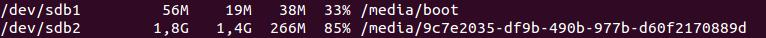
\includegraphics[scale=0.7]{images/InstalRasp1.jpeg}
\end{center}
Se deben desmontar las dos particiones, tanto la \textit{/dev/sdb1} como la \textit{/dev/sdb2}:
\begin{verbatim}
           umount /dev/sdb1
           umount /dev/sdb2
\end{verbatim}
Descargada la imagen a instalar, por ejemplo en el Escritorio, se procede con:
\begin{verbatim}
    sudo dd bs=4M if=~/Escritorio/2013-07-26-wheezy-raspbian.img of=/dev/sdb
\end{verbatim}
Pasados unos minutos ya se tiene la SD grabada con el sistema operativo Raspbian.
\subsubsection*{Configuración de la Raspberry}
Para poder comunicar la RPi con la IMU MPU-6050 por I2C es necesario configurar el sistema. Primero es necesario instalar los drivers mas relevantes. Del archivo
\begin{verbatim}
           sudo nano /etc/modules
\end{verbatim}
se añaden las siguientes dos líneas al final del archivo:
\begin{verbatim}
           i2c-bcm2708
           i2c-dev
\end{verbatim}
En el archivo blacklist:
\begin{verbatim}
           sudo vi /etc/modprobe.d/raspi-blacklist.conf
\end{verbatim}
las siguientes dos líneas deben empezar con un signo \# (de comentario):
\begin{verbatim}
           #blacklist spi-bcm2708
           #blacklist i2c-bcm2708
\end{verbatim}
Para conectar el sensor, es necesario seguir primero el conexionado:

\begin{figure}[h!]
\begin{center}
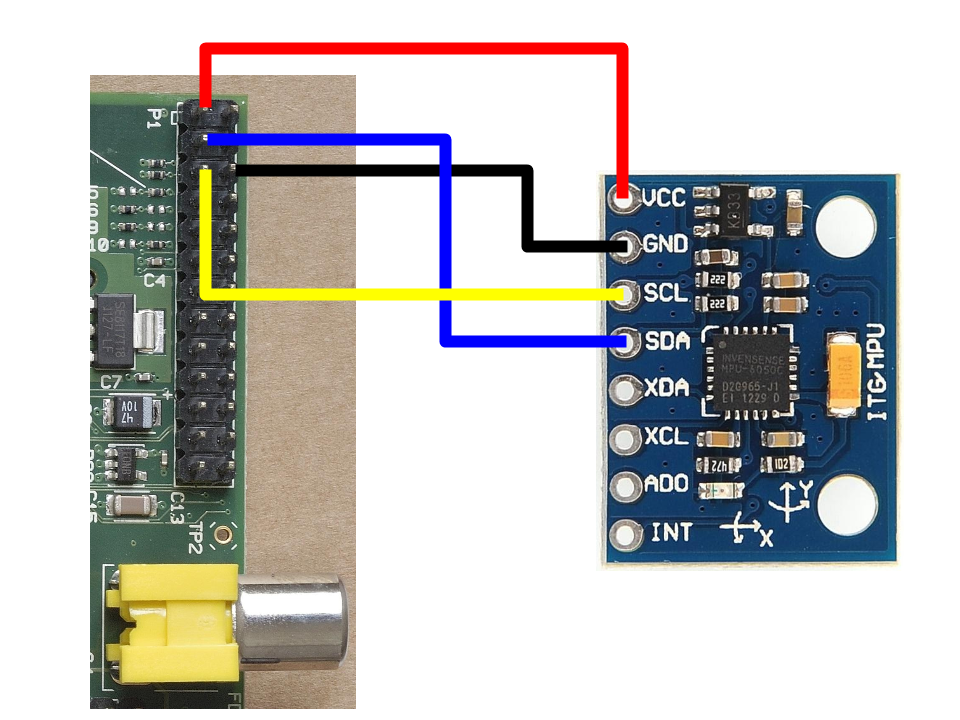
\includegraphics[scale=0.2,viewport=0 200 800 720,clip]{images/ConSens.jpg}
\caption{Conexión por I2C entre MPU-6050 y RPi}
\end{center}
\end{figure}


Es decir
\begin{itemize}
\item Pin 1-3.3V se conecta a VCC.
\item Pin 3-SDA se conecta a SDA
\item Pin 5-SCL se conecta a SCL
\item Pin 6-Ground se conecta a GND
\end{itemize} 
Es necesario instalar el paquete $i2c-tools$:
\begin{verbatim}
           sudo apt-get install i2c-tools
\end{verbatim}
Para ver el sensor se escribe:
\begin{verbatim}
           sudo i2cdetect -y 1
\end{verbatim}
El resultado es 

\begin{figure}[h!]
\begin{center}
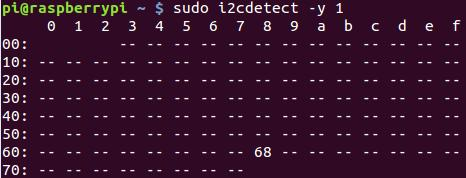
\includegraphics[scale=0.7]{images/i2cdetect.jpg}
\caption{Detección del sensor MPU-6050}
\end{center}
\end{figure}
que es el dispositivo que corresponde al MPU-6050.

\subsubsection*{Librería wiringPi}
Se utiliza esta librería \cite{wiringPi} como a interfaz del GPIO (General Porpouse Input Output). Permite, por tanto, leer las consignas y sensores y generar las acciones de control. 
La instalación y descripción de la librería esta explicado en la página web incluida en la bibliografía.

\newpage
\subsection*{Anexo 3: Filtro de Kalman}
\newpage
\subsection*{Anexo 4: Identificación de los parámetros del Quadcopter}
%% Inercias, longitud brazos, motores (fuerza e intensidad)
Para poder trabajar en particular con el Quadcopter construido es necesario saber qué lo caracteriza o distingue de los demás. Parámetros relevantes y necesarios que se utilizan en el modelo implementado en Simulink deben ser, entonces, medidos para que se simule el mismo aparato con iguales características. \\

Se consideran relevantes la matriz de inercias, la longitud de los brazos  $l$ y la la fuerza e intensidad (consumo) de los motores respecto a la señal $PWM$ con que se controlan.\\

Con este conjunto de parámetros se considera que el Quadcopter está totalmente definido y puede obtenerse la ley de control.

\subsubsection*{Inercias}

Como se ha comentado en la sección \ref{def}, se supone que el Quadcopter es un rotor esférico, y por tanto de su tensor de inercia todos los productos de inercia serán nulos. Se tendrá entonces una matriz diagonal como tensor. En este apartado, entonces, el objetivo será la medición de los dos momentos de inercia $I_{xx}$ y $I_{yy}$, correspondientes a los ángulos $Roll$ y $Pitch$. Para ello se usa una bancada compuesta por un muelle de constante de torsión $D$ conocida del que cuelga el quadcopter. De querer determinar el momento de inercia $I_{xx}$, se cuelga desde uno de los extremos del eje $x$, tal y como se observa en la figura \ref{Quad_spring}

\begin{figure}[h!]
\begin{center}
\begin{tikzpicture}
\draw[decoration={aspect=0.3, segment length=2mm, amplitude=3mm,coil},decorate] (0,5) -- (0,2); 

\path[draw, line width=5pt,color =black] (0,0) -- (0,2);
\path[draw, line width=5pt,color =black] (-0.8,1.4) -- (0.8,0.6);

\path[draw, line width=5pt,color =black] (0.05,0.05) -- (-0.3,-0.18);
\path[draw, line width=5pt,color =black] (0.05,2.05) -- (-0.3,1.82);
\path[draw, line width=5pt,color =black] (-0.75,1.4) -- (-1.1,1.2);
\path[draw, line width=5pt,color =black] (0.85,0.62) -- (0.5,0.42);

\path [draw, line width=1pt] (-1,3) -- (-1,2);
\path [draw, line width=1pt] (-1.2,2.2) -- (-1,2) -- (-0.8,2.2);

\path[draw] (-1.3,2.5) node (nodeC) {\large $\dot{\Omega}$};
\path[draw] (0.7,3.5) node (nodeC) {\large D};

\path[draw,line width=1pt,dotted, color=black](-1.6,1.8) -- (1.6,0.2);
\path[draw,line width=1pt,dotted, color=black](-1,0.34) -- (1,1.66);
\path[draw,line width=1pt,dotted, color=black](0,3) -- (0,-1);

\path[draw,line width=1pt] (0,-0.5) -- (0,-1);
\path[draw,line width=1pt] (-0.1,-0.8) -- (0,-1) -- (0.1,-0.8);
\path[draw] (0.4,-0.7) node (nodeC) {\large x};
\path[draw] (-0.3,0.8) node (nodeC) {\large o};

\fill [pattern = north east lines] (-1,5) rectangle (1,5.2);
\draw[thick] (-1,5) -- (1,5);
\end{tikzpicture}
\end{center}
\caption{Bancada para la determinación de las inercias}
\label{Quad_spring}
\end{figure}

Para un sólido rígido se tiene que 

\begin{equation}
\mathbf{M}=\frac{d\mathbf{L_{o}}}{dt}
\end{equation}

donde $\mathbf{M}$ es el momento resultante y $\mathbf{L_{o}}$ es el momento cinético o angular aplicado en el punto $o$, que en este caso corresponde al centro de gravedad del cuerpo. Éste se expresa como

\begin{equation}
\mathbf{L_{o}}=\mathbf{I}\dot{\mathbf{\Omega}}
\end{equation}

El momento resultante puede expresarse entonces de la forma 

\begin{equation}
\mathbf{M}=\frac{d(\mathbf{I}\dot{\mathbf{\Omega}})}{dt}=\mathbf{I}\ddot{\mathbf{\Omega}}=\left[ \begin{array}{ccc}
I_{xx} & 0 & 0 \\
0 & I_{yy} & 0 \\
0 & 0 & I_{zz} \\
\end{array} \right]\left[ \begin{array}{c}
\ddot{\Omega}_{x} \\
\ddot{\Omega}_{y} \\
\ddot{\Omega}_{z} \\
\end{array} \right]=\left[ \begin{array}{ccc}
I_{xx} & 0 & 0 \\
0 & I_{yy} & 0 \\
0 & 0 & I_{zz} \\
\end{array} \right]\left[ \begin{array}{c}
\ddot{\Omega} \\
0 \\
0 \\
\end{array} \right] = I_{xx} \ddot{\Omega}
\label{53}
\end{equation}

en suponer que el tensor de inercia no varía con el tiempo. Se asume 
que el eje de rotación $\dot{\Omega}$ pasa por el centro de masas, de lo contrario debería aplicarse el teorema de Steiner. Para el muelle se tiene que, según la ley de Hooke

\begin{equation}
M=-D \cdot \Omega
\label{54}
\end{equation}

donde $\mathbf{\Omega}$ es el ángulo girado en la dirección longitudinal del muelle. Igualando las expresiones \ref{53} y \ref{54} se llega a 

\begin{equation}
-D \cdot \Omega = I_{xx}\ddot{\Omega}\quad \Longrightarrow \quad \ddot{\Omega}+\frac{D}{I_{xx}}\Omega =0 
\end{equation}

La solución de la ecuación anterior es el de un oscilador armónico de periodo 

\begin{equation}
T=2\pi \sqrt{\frac{I_{xx}}{D}}
\end{equation}

Ésto se cumple en oscilaciones pequeñas cercanas al punto de equilibrio, donde $\Omega=\dot{\Omega}=\ddot{\Omega}$. Por lo tanto, el periodo de una oscilación es suficiente para poder calcular el momento de inercia en estar directamente relacionados. Para obtener resultados más precisos se medirá el tiempo varias veces. \\

Para calcular la constante de torsión del muelle se le ha sometido a ensayo, sometiéndolo a diferentes deformaciones elásticas y observando con qué momento éste respondía:
\begin{center}
\begin{tabular}{|c|c|c|}
\hline
$\mathbf{\Omega}$(º) & $\mathbf{M}$($g \cdot 10cm$) & $\mathbf{M}$($N \cdot m$) \\
\hline 
\hline 
30 & 33 & 0.0323 \\
45 & 46 & 0.0451 \\
60 & 62 & 0.0608 \\
90 & 93 & 0.0912 \\
\hline 
\end{tabular}
\end{center}

En calcular la relación entre ambas magnitudes para obtener la constante de torsión del muelle, por regresión lineal se obtiene que la pendiente es de $1.0095\>\>g\cdot10cm/grad$. La constante entonces puede expresarse en unidades del Sistema Internacional como 

\begin{equation}
D=1.0095 \>\> \frac{g\cdot10cm}{grad}\cdot\frac{9.81 \>\> N}{1000 \>\> g} \cdot \frac{1 \>\> m}{100 \>\> cm} \cdot \frac{360 \>\> grad}{2\pi \>\> rad} = 0.0567 \>\> \frac{Nm}{rad}
\end{equation}

En hacer oscilar el Quadcopter en el eje $x$ se obtiene:

\begin{center}
\begin{tabular}{|c|cccc|c|c|}
\hline
\textbf{Eje} & \multicolumn{4}{c|}{\textbf{Muestras}(s)} & \textbf{Media}(s) & \textbf{Momento de inercia}($kg \cdot m^{2}$) \\
\hline
\multirow{4}{*}{$x$} & 2.3 & 2.3 & 2.5 & 2.2 & \multirow{4}{*}{2.35} & \multirow{4}{*}{$7.932\cdot 10^{-3}$} \\
& 2.3 & 2.4 & 2.5 & 2.4 & & \\
& 2.4 & 2.3 & 2.3 & 2.4 & & \\
& 2.3 & 2.4 & 2.3 & 2.3 & & \\
\hline
\multirow{4}{*}{$y$} & 2.4 & 2.3 & 2.2 & 2.4 & \multirow{4}{*}{2.31} & \multirow{4}{*}{$7.664\cdot 10^{-3}$} \\
& 2.2 & 2.4 & 2.3 & 2.2 & & \\
& 2.4 & 2.3 & 2.3 & 2.4 & & \\
& 2.3 & 2.3 & 2.3 & 2.3 & & \\
\hline
\end{tabular}
\end{center}

y por tanto se obtiene que $I_{xx}=7.931\cdot 10^{-3} \>\> kg \cdot m^{2}$ y $I_{yy}=7.664\cdot 10^{-3}\>\> kg \cdot m^{2}$.

\subsubsection*{Longitud de brazo}

Queda especificado en el modelo del Frame elegido que es de $33 \>\> cm$ la distancia de motor a motor, es decir, de la diagonal principal. La longitud que se considera es de $l=16.5 \>\> cm$.

\subsubsection*{Motores}
Para poder controlar la planta es necesario saber cómo responden los actuadores para realizar un control preciso. De éstos se deben conocer qué fuerza y momento proporcionan, así como el consumo de energía, dado un PWM. 
Para obtener una curva de la fuerza respecto del PWM se pesa con una balanza la acción del motor. La rudimentaria bancada que se tiene para tal objetivo es un codo articulado en el eje de tal manera que la distancia del eje del motor al fulcro y de éste a la balanza sea la misma (en este caso de 12 cm):

\begin{figure}[h!]
\begin{center}
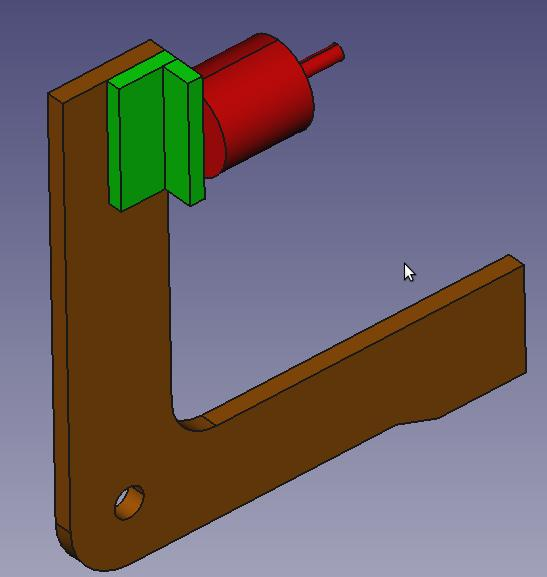
\includegraphics[scale=0.4]{images/bancada1.jpeg}
\caption{Bancada para el estudio del motor}
\end{center}
\end{figure}
Las partes están hechas de madera (parte marrón) y plástico ABS (parte verde). Toda la estructura se sujeta a unas maderas:

\begin{figure}[h!]
\begin{center}
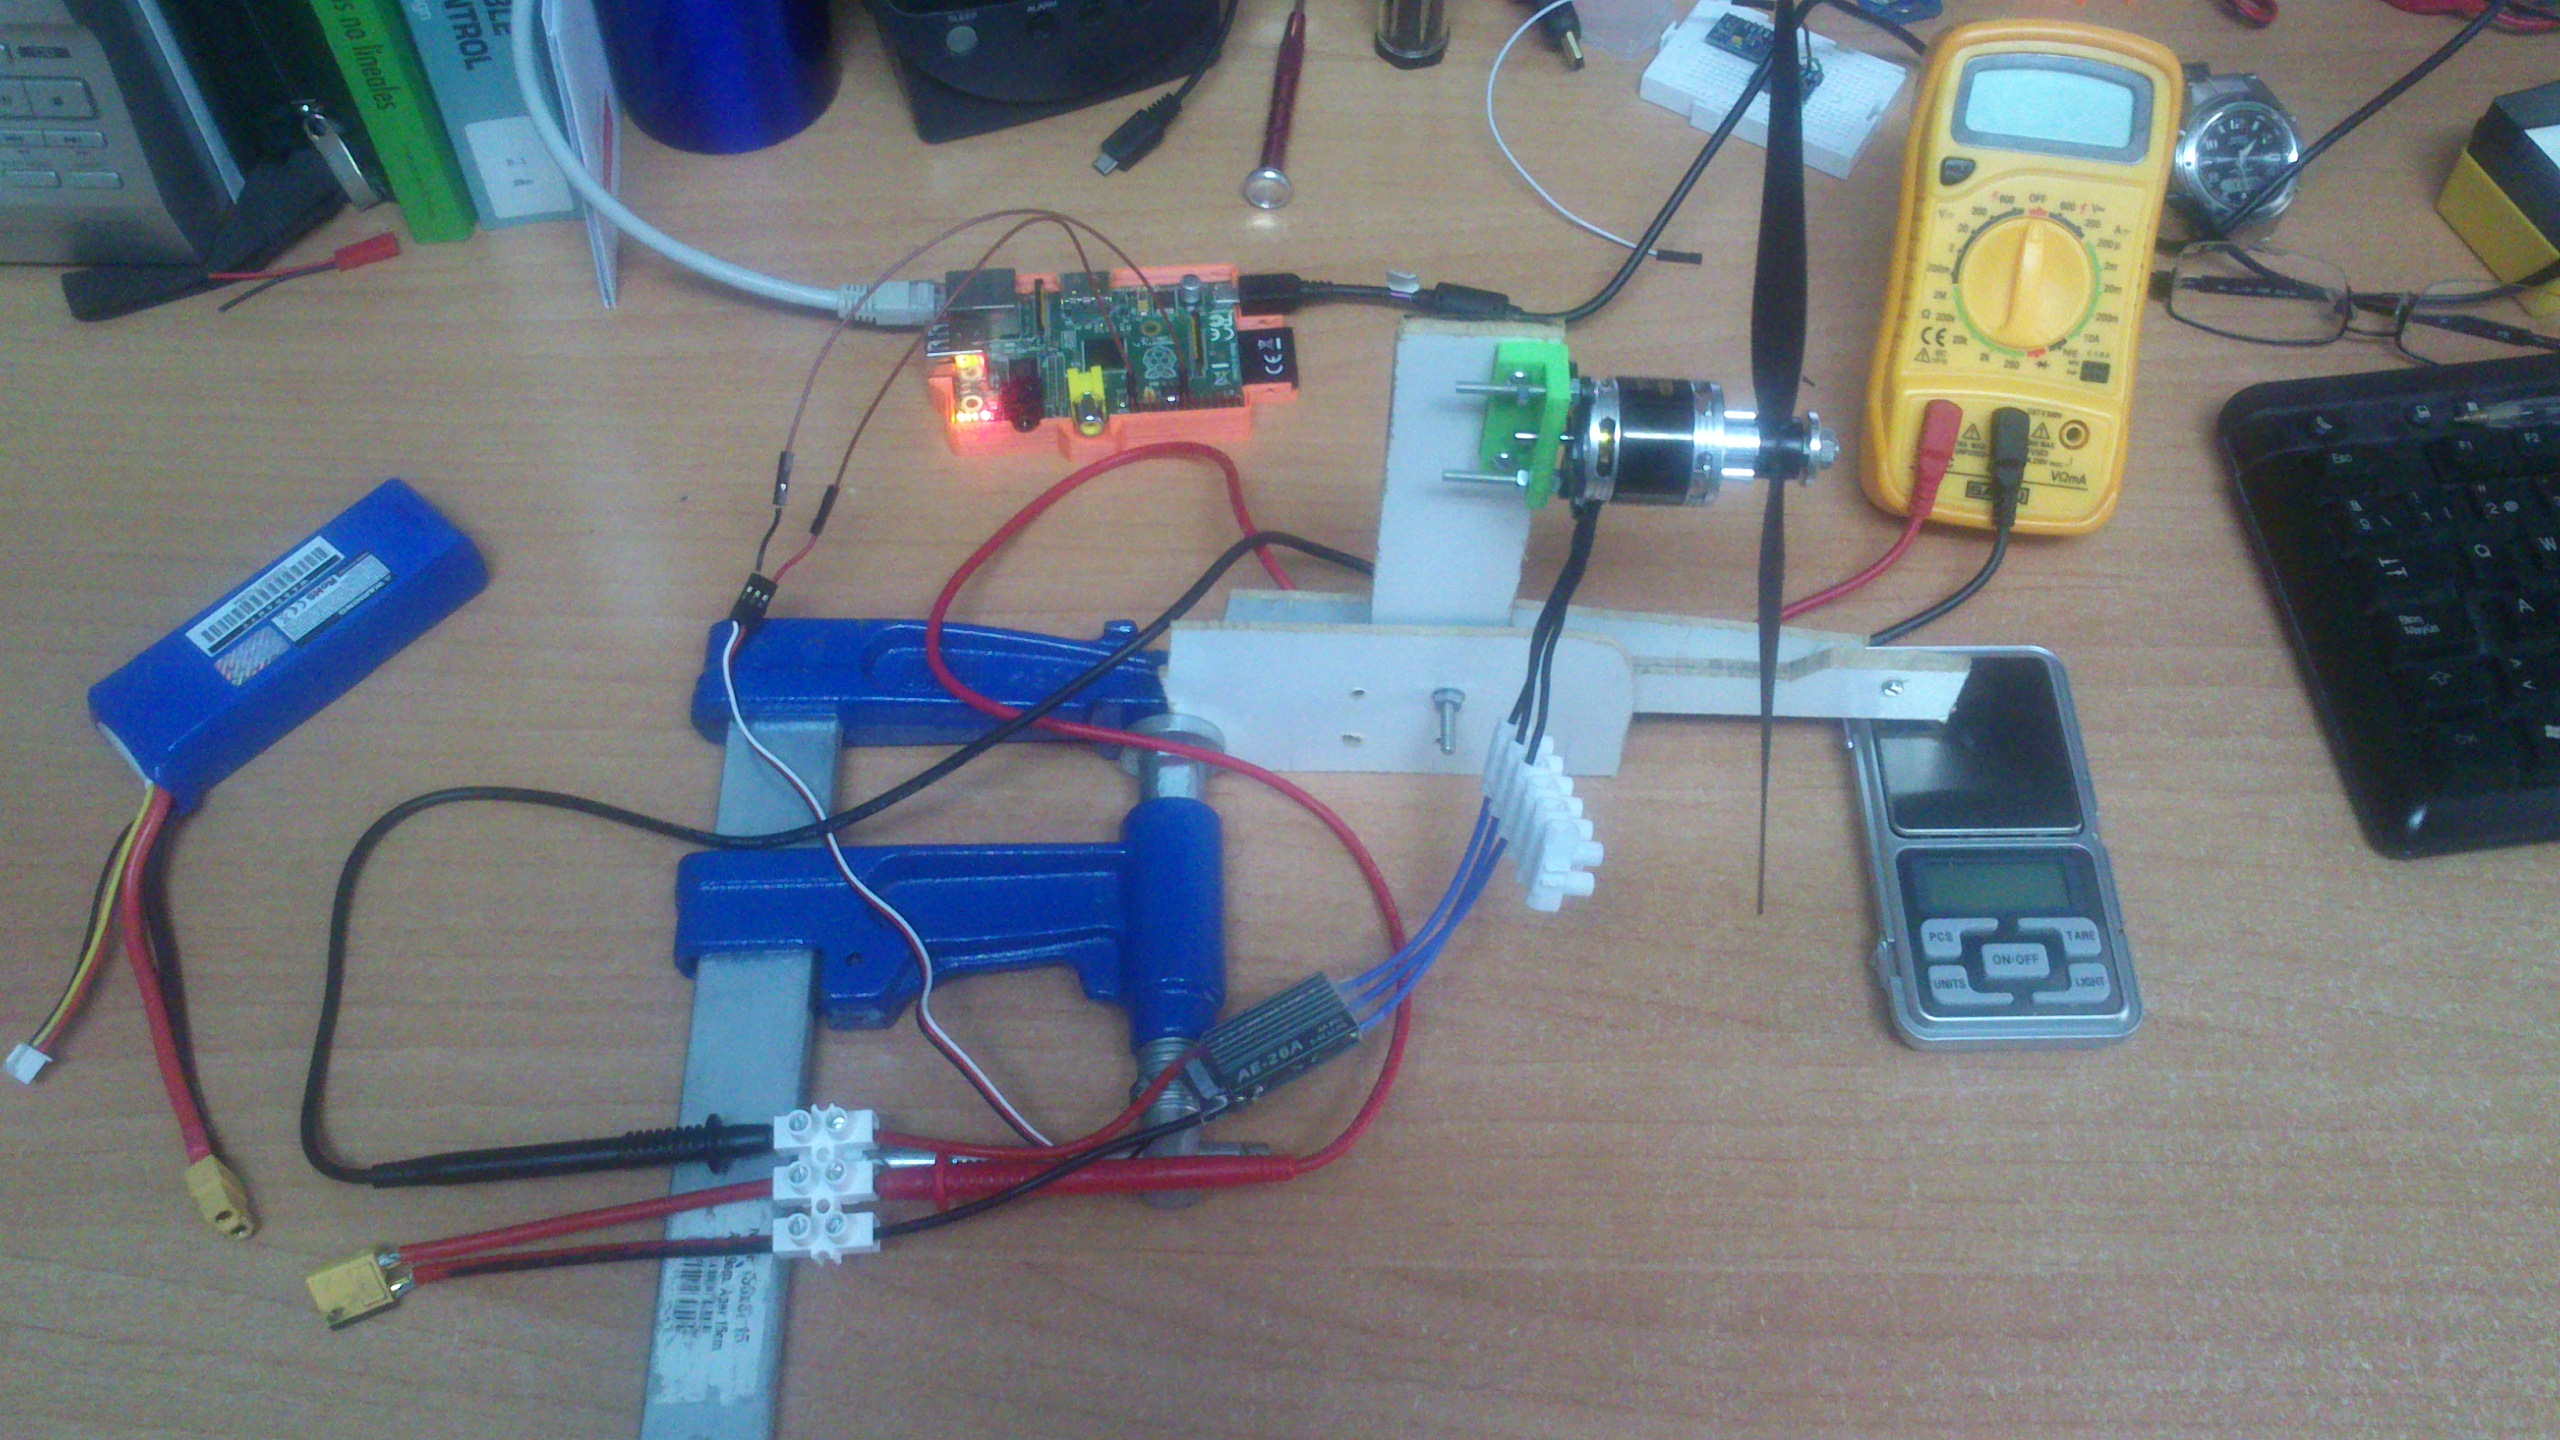
\includegraphics[scale=0.09]{images/montaje.jpg}
\caption{Montaje para el estudio del motor}
\end{center}
\end{figure}

Se transmite al ESC a qué velocidad se debe hacer funcionar el motor des de la Raspberry Pi por medio de una señal PWM. El programa que se ejecuta para hacer las pruebas es:

\begin{lstlisting}[language=C]
#include <stdio.h>
#include <termios.h>
#include <wiringPi.h>
#include <unistd.h>

#define PIN 2 // pin 13

int main(void){

        int i,p;
        wiringPiSetup();

        pinMode(PIN,OUTPUT);
        digitalWrite(PIN,LOW);

        for(i=0;i<=100;i+=5){
                for(p=0;p<250;p++){
                        digitalWrite(PIN,HIGH);
                        delayMicroseconds(950+i*10);
                        digitalWrite(PIN,LOW);
                        delayMicroseconds(19050-i*10);

                        printf("PWM(i): %d \t h:%d \n",i,p);
                }
        }
        return 0;
}
\end{lstlisting}

\vspace{0.75cm}
Se obtiene una lectura de fuerza y  de intensidad por cada incremento del 0.25\% del PWM enviado al Variador. Las lecturas que se obtienen son: 

\begin{center}
\begin{tabular}{|c|c|c|}
\hline
\textbf{PWM(\%)} & \textbf{Fuerza(g)} & \textbf{Intensidad(A)} \\
\hline
\hline
5    &	  0 &   0 \\
\hline
5,25 & 0,25 &  13 \\
\hline
5,5	 &  0,5 &  38 \\
\hline
5,75 &  0,9 &  74 \\
\hline
6    & 1,38 &  98 \\
\hline
6,25	 &  1,8 & 128 \\
\hline
6,5  &	2,4 & 158 \\
\hline
6,75 & 	2,9 & 191 \\
\hline
7    &	3,5 & 215 \\
\hline
7,25 &  	  4	& 250 \\
\hline
7,5  & 	4,6 & 277 \\
\hline
7,75	 &  5,5 & 318 \\
\hline
8    &	6,5	& 360 \\
\hline
8,25 &    8 & 400 \\
\hline
8,5  & 9,15 & 450 \\
\hline
\end{tabular}
\end{center}
Graficado:

%\begin{figure}[h!]
%\begin{center}
%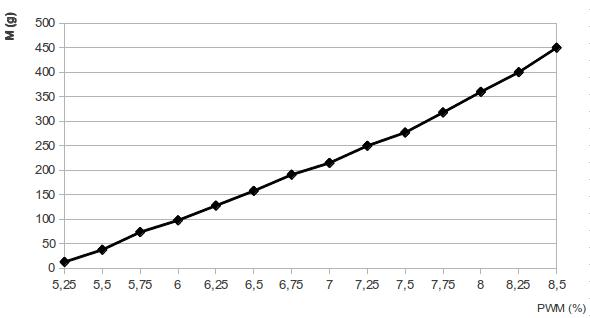
\includegraphics[scale=0.8]{images/MvsPWM.jpeg}
%\caption{Relación entre la fuerza (en gramos) y el PWM}
%\end{center}
%\end{figure}

\begin{figure}[ht]
\begin{center}
\begin{tikzpicture}
\path[draw] (11,-0.5) node {PWM(\%)};
\path[draw] (-0.6,6.5) node {M(g)};
\begin{axis}[width=12cm,height=6cm,xmin=5,ymin=0]

\addplot[color=black,solid,thick,mark=*, mark options={fill=white}] 
    coordinates {
%         (2211, 1110)
%         (6164, 4168)
%         (11610, 36335)
			(5,0)
			(5.25,13)	
			(5.5,38)
			(5.75,74)
			(6,98)
			(6.25,128)
			(6.5,158)
			(6.75,191)
			(7,215)
			(7.25,250)
			(7.5	,277)
			(7.75,318)
			(8,360)
			(8.25,400)
			(8.5	,450)
        }; 
        


% \path[draw] [domain=5:10,red] plot ({\x},{32.575824*\x-32.175});        
%\addplot[red, thick] {5,8.5}(x,32.575824*x-32.175); 
% \node [above] at (axis cs:  2211,  1110) {$32h$};
% \node [below] at (axis cs:  6164,  4168) {$x_1$};
% \node [left ] at (axis cs: 11610, 36335) {$x_1-PPL_{18}$};
% \path[draw] [scale=5,red] plot ({\x},{32.575824*\x-32.175});      
\end{axis}
% \draw[red] plot[samples=200,domain=-1:2] function {x**2};
\end{tikzpicture}
\caption{Relación entre la fuerza (en gramos) y el PWM}
\end{center}
\end{figure}


\begin{tikzpicture}
%\foreach \Point in {(5,0), (5.25,13), (5.5,38), (5.75,74), (6,98)}{
%    \node at \Point {\textbullet};
%}
\begin{axis}[width=10cm,height=6cm, xmin=5]
%    xmin=-10, xmax=10,
%    ymin=-10, ymax=10,
%    xtick=\empty, ytick=\empty
]
\addplot[color=black,solid,thick,mark=*, mark options={fill=white}] 
    coordinates {
%         (2211, 1110)
%         (6164, 4168)
%         (11610, 36335)
			(5,0)
			(5.25,13)	
			(5.5,38)
			(5.75,74)
			(6,98)
			(6.25,128)
			(6.5,158)
			(6.75,191)
			(7,215)
			(7.25,250)
			(7.5	,277)
			(7.75,318)
			(8,360)
			(8.25,400)
			(8.5	,450)
        }; 
\addplot[dashed] {1};
\end{axis}
\end{tikzpicture}

En el eje de les abscisas el PWM(\%) es entre el 5\% y el 10\% de la señal enviada, que corresponden al mínimo y máximo del motor. Para un PWM elevado la fuerza era demasiado grande y no se prevé que se haga funcionar al sistema en semejantes condiciones de trabajo, no se estudia. 

Se ve una relación proporcional del PWM con la fuerza generada. Se considera que una regresión lineal será suficiente. Se obtiene que la fuerza $f(PWM)$ del motor será:
$$f=32.5758 \cdot PWM(\%)-32.1758$$
con un coeficiente de determinación en la regresión de  $R^2=0.9929$. Este resultado facilita el problema en ser una relación suficiente sencilla.

Para la intensidad se tiene una relación tan amigable como en el caso anterior, pero como no sera caso de estudio,solo se verá una aproximación de lo que puede llegar a consumir cada motor para asegurar una autonomía de vuelo no irrisoria. Resulta
% \newpage

%\begin{figure}[!h]
%\begin{center}
%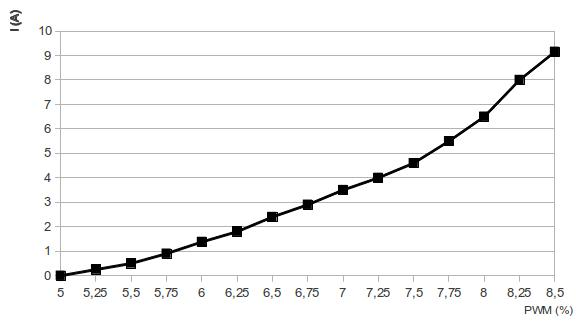
\includegraphics[scale=0.8]{images/IvsPWM.jpeg}
%\caption{Relación entre la corriente consumida y el PWM}
%\end{center}
%\end{figure}

\begin{figure}[ht]
\begin{center}
\begin{tikzpicture}
\begin{axis}
\addplot [color=black,solid,thick,mark=*, mark options={fill=white}] coordinates {
%         (2211, 1110)
%         (6164, 4168)
%         (11610, 36335)
			(5,0)
			(5.25,13)	
			(5.5,38)
			(5.75,74)
			(6,98)
			(6.25,128)
			(6.5,158)
			(6.75,191)
			(7,215)
			(7.25,250)
			(7.5	,277)
			(7.75,318)
			(8,360)
			(8.25,400)
			(8.5	,450)
        }; 
% \addplot[red, thick] (x,32.575824*x-32.175);        
% \node [above] at (axis cs:  2211,  1110) {$32h$};
% \node [below] at (axis cs:  6164,  4168) {$x_1$};
% \node [left ] at (axis cs: 11610, 36335) {$x_1-PPL_{18}$};
\addplot [domain=-10:10, samples=2, dashed] {32.575824*x-32.175};
\end{axis}
\end{tikzpicture}
\end{center}
\end{figure}

Como en el punto de equilibrio cada motor soporta una cuarta parte del peso, el PWM debería corresponder al de una fuerza de $m_{Quadcopter}\cdot g/4\approx0.225$kg. El consumo correspondiente es de $3.5$A aproximadamente. Entre los cuatro motores se consumirán $3.5 \cdot 4=14$A. Como que la batería es de 2200mAh se supone una autonomía de 7 minutos aproximadamente. 

\end{document}